% ---
% Capitulo Análises Realizadas
% ---
\chapter{Análises Preliminares}\label{chap:analises-preliminares}
% META: 15p.

\section{Periodicidade e Objetivos da Pesquisa Origem Destino}\label{sec:period-obj}

A Pesquisa Origem Destino (Pesquisa OD) é realizada a cada dez anos pela Companhia do Metropolitano de São Paulo (Metrô-SP), a partir de 1967. Assim, até hoje foram realizadas cinco Pesquisas OD realizadas (1967, 1977, 1987, 1997 e 2007), das quais este trabalho abrangerá as quatro últimas, cobrindo uma janela temporal de 30 anos. O intervalo de dez anos foi considerado pelo Metrô-SP muito longo mediante as rápidas transformações no espaço urbano; assim, em 2002 e em 2012 foram feitas Pesquisas de Aferição, com menor amostragem e zonas mais agregadas. Cabe esclarecer que estas pesquisas de aferição não serão objeto de análise do presente estudo.

A Pesquisa OD nasceu com a missão de compor uma base de dados que servisse de suporte a decisões de planejamento de transporte urbano na Região Metropolitana de São Paulo, que hoje abarca 38 municípios, além de São Paulo. Hoje, além de cumprir esse papel, também é ferramenta de suporte para o planejamento urbano de maneira mais sistêmica, bem como para a formulação de políticas públicas segmentadas, nas áreas de educação, saúde e segurança pública, por exemplo \cite{MANUALOD2007}.

\section{Descrição da Pesquisa OD}\label{sec:descricao-OD}

A Pesquisa OD é composta de duas partes complementares, a saber, a Pesquisa Domiciliar e a Pesquisa de Linha de Contorno. A Pesquisa Domiciliar tem como escopo as viagens internas à Região Metropolitana de São Paulo (RMSP), nela são escolhidos domicílios por amostragem, cujo critério será melhor discutido adiante, em que todos habitantes respondem a um questionário estruturado referente às viagens feitas no dia útil anterior à pesquisa. Já a Pesquisa de Linha de Contorno monitora pontos de entrada e saída (limites) da RMSP a fim de captar as viagens com origem dentro da RMSP e destino fora, vice-versa, ou ainda viagens que a atravessam. O presente trabalho tem como foco as viagens feitas internamente à RMSP, portanto, as bases de dados consideradas serão apenas aquelas advindas das Pesquisas Domiciliares.

A Pesquisa OD considera a dimensão espacial dos deslocamentos considerando as zonas de origem e de destino. Tais zonas tiveram seus limites alterados e área total expandida desde 1967. Na Tabela \ref{tab:carac-dados} é possível observar quantos municípios da RMSP foram envolvidos em cada pesquisa e em quantas zonas eram divididos. A coorespondência entre as diversas zonas é feita por uma unidade de compatibilização chamada Unidade de Correspondência de Zona (UCOD), em relação às quais todas zonas têm referência. Para que seja possível realizar uma análise de evolução temporal conjugando dados de diversas OD é preciso organizar todas informações de maneira coerente, assim, é apresentado no Anexo \ref{chap:anexo_ucod} as 67 UCOD  com as respectivas zonas correspondentes para 1977, 1987, 1977 e 2007. Para tal consolidação ser feita, parte das informações foi recebida do Metrõ-SP e parte foi fruto de compilação própria.


\begin{table}[htb]
    \IBGEtab{%\renewcommand{\arraystretch}{1.5}%%\ABNTEXfontereduzida%
	    \renewcommand{\arraystretch}{1.5}
        \caption{Caracaterísticas Amostrais das Pesquisas OD}
		\label{tab:carac-dados}
    }{%
	    \begin{tabular}{P{2.00cm} P{4.0cm} P{4.0cm}}
            \toprule
	           \headerTabCenterCell{Ano} &
   	           \headerTabCenterCell{Zona} &
		       \headerCell{Municípios da RMSP}\\
		    \midrule \midrule
				1967&
				15&
		        206\\
		    \midrule
		        1977&
		        27&
		        243\\
		    \midrule
		        1987&
		        39&
		        254\\
		    \midrule
		        1997&
		        39&
		        389\\    
		    \midrule
		        2007&
		        39&
		        460\\    
			\bottomrule	
		\end{tabular}
    }{%
		\fonte{Compilação a partir de {\cite{OD77,OD87,OD97,OD07}}}
		}
\end{table}


\subsection{Dados Coletados}\label{subsec:dados-coletados}

A Pequisa OD coleta dados referentes a viagens, indivíduos, famílias e domicílios, o que possibilita buscar relações entre características de deslocamentos e de indivíduos (e respectivas famílias e domicílios), e também características socioeconômicas. A amostra de domicílios é do tipo estratificada por faixas de consumo de energia elétrica - isso se dá por dois fatores: (i) as concessionárias possuem uma bases cadastrais de registro de domicílios mais confiáveis e representativas; (ii) ``o consumo de energia elétrica tem correlação com a renda familiar, que por sua vez tem correlação com o número de viagens da família'' \cite[p.10]{MANUALOD2007}. Esse esquema de amostragem estratificada buscou, em todos anos obter npível de confiança de 95\%. Nas zonas em que não foi possível utilizar esse arranjo, foi feita amostra causal simples, com erros em tornode 7,5\%. Na Tabela \ref{tab:tam-amostra} é possível observar algum dados relativos às amostras.
%TODO confirmar esse 7.5% com Emilia, bem como de o IC foi 95% sempre

Definido o tamanho da amostra total, define-se o tamanho de amostra para cada zona e a partir daí, procede-se um sorteio de endereços por fiaxa de consumo energético - etapa esta realizada pelas concessionárias, que fornecem ao Metrô-SP apenas os endereços dos domicílios selecionados, além de alguns adicionais para substituição caso necessário. Os selecionados recebem comunicação oficial por carta do Metrô-SP contendo as informações pertinentes à pesquisa. Quando no domicílio, os(as) pesquisadores(as) aplicam o questionário a todas pessoas que moram ali.


\begin{table}[htb]
    \IBGEtab{%\renewcommand{\arraystretch}{1.5}%%\ABNTEXfontereduzida%
	    \renewcommand{\arraystretch}{1.5}
        \caption{Caracaterísticas Gerais das Pesquisas OD}
		\label{tab:tam-amostra}
    }{%
	    \begin{tabular}{P{2.00cm} P{4.0cm} P{4.0cm} P{4.0cm}}
            \toprule
	           \headerTabCenterCell{Ano} &
   	           \headerTabCenterCell{Domicílios} &
		       \headerCell{Pessoas entrevistadas do sexo feminino} &
   		       \headerCell{Pessoas entrevistadas do sexo masculino}\\
		    \midrule \midrule
				1967&
				Não disponível&
				Não disponível&
		        Não disponível\\
		    \midrule
				1977&
				26.132&
				55.868&
		        52.161\\
		    \midrule
				1987&
				26.070&
				57.637&
		        53.176\\
		    \midrule
				1997&
				23.841&
				51.454&
		        57.326\\
		    \midrule
		        2007&
		        29.957&
		        53.561&
		        51.732\\    
			\bottomrule	
		\end{tabular}
    }{%
		\fonte{Compilação a partir de \cite{OD77,OD87,OD97,OD07}}
		}
\end{table}

A coleta, consistência e digitação do dados são de responsabilidade de institutos de pesquisa contratados pelo Metrô-SP e que variaram ao longo do tempo. Após a consolidação primeira do banco de dados, são aplicados fatores de expansão aos resultados amostrais. Primeiro aplica-se aos domicílios, às famílias e às pessoas pesquisadas segundo as expressões \eqref{eq:fator-expansao-dom}, \eqref{eq:fator-expansao-fam} e \eqref{eq:fator-expansao-pess}. Depois determina-se o fator de expansão das viagens. As viagens de quem usaou o modo metrô são expandidas levando em consideração a entrada de passageiros no sistema Metrô-SP na data de referência da pesquisa. Situação análoga ocorre com o trem metropolitano. As viagens de quem usou outro modo que não metrô e/ou trem teve seu fator de expansão de viagens determinado pelo total de passageiros transportados pelo sistema de ônibus (em 2007 foram utilizados os dados provenientes de Bilhete Único da SPTrans).

\begin{equation}\label{eq:fator-expansao-dom}
\mbox{Fator de expansão de domicílio}_i = \frac{\mbox{Total de domicílios da zona}_i}{\mbox{domicílios da amostra da zona}_i}
\end{equation}

%Referênciando a equação \ref{eq:fator-expansao} ou usando \eqref{eq:fator-expansao}.

\begin{equation}\label{eq:fator-expansao-fam}
\mbox{Fator de expansão da família}_i = \frac{\mbox{Total de famílias da zona}_i}{\mbox{famílias da amostra da zona}_i}
\end{equation}

\begin{equation}\label{eq:fator-expansao-pess}
\mbox{Fator de expansão da pessoa}_i = \frac{\mbox{Total de pessoas da zona}_i}{\mbox{pessoas da amostra da zona}_i}
\end{equation}

Vale fazer algumas considerações acerca da renda familiar. Nem todas pessoas respondem qual é a renda familiar, e como trata-se de uma das informações mais importantes para descrever o comportamento das pessoas \hl{FALTA REF} nestes casos, a renda é atribuída, mas não sem critério. A atribuição da renda familiar tem origem em expressão de regressão linear feita a partir de pontuação estabelecida por algum critério nacional
\footnote{Em 2007 foi usado o Critério Brasil, criado em 1996 pela Associação Nacional de Empresas de Pesquisa, e adotado por seus associados como padrão de segmentação da população em categorias de capacidade de consumo. Fonte: \url{http://www.abep.org/new/criterioBrasil.aspx}}, que variou ao longo do tempo - tais informações podem ser vistas no Quadro \ref{qua:atrib-renda}. 
A função dessas regressões é estimar o poder de compra das pessoas, agrupando-as em classes econômicas, a partir da posse de bens de consumo e do grau de instrução ''do chefe da família''. Nesses critérios de classificação econômica existe a orientação de que a categoria automóvel não deve considerar táxis, vans, \emph{pickups} usadas para fretes ou qualquer veículo usada para atividades profissionais, nem tampouco devem ser considerados veículos de uso misto (lazer e profissional) \cite{CRITERIOBRASIL}. Essa mesma orientação em relação aos automóveis é feita pelos manuais das Pesquisas OD \cite{OD77, OD87, OD97, OD07} tornando o conjunto coerente.
Nas famílias em que não se obteve nem declaração da renda, nem informações suficientes sobre bens de consumo, a renda foi atribuída à família a partir da mediana da zona a que pertencia e com mesmo grau de instrução da ``chefe da família''.

\begin{quadro}[htb]
    \IBGEtab{
        \renewcommand{\arraystretch}{1.5}
        \ABNTEXfontereduzida
        \caption[Dados para atribuição de renda familiar]{\label{qua:atrib-renda}Dados para atribuição de renda familiar}
	}{%
        \begin{tabular}{|P{2.0cm}|P{2.00cm}|P{5.00cm}|P{3.50cm}|}
           \hline
		       \headerCenterCell{Ano} & 
		       \headerCenterCell{Mês de Referência} & 
		       \headerCenterCell{Critério de Classificação} & 
		       \headerCenterCell{Índice de Correção*}\\ 
		    \hline\hline
		        1977&
		    	\hl{aguardando resposta Emilia}&
		        Função do Salário Mínimo&
		        \hl{??}\\
		    \hline
		    	1987&
		        setembro&
		        Critério ABA/ABIPMEPE (análogo ao Critério Brasil)&
		        0,000010223607163\\
		    \hline
		    	1997&
		        outubro&
		        Critério Brasil (ABIPMEPE)&
		        1.419,28\\
		    \hline
		    	2007&
		        outubro&
		        Critério Brasil (ABEP)&
		        2.755,34\\
			\hline
		\end{tabular}
	}{%
		\fonte{Compilação de informações obtidas por meio de correspondência eletrônica com Metrô-SP}
		\nota{Não existem informações de INPC anteriores a 1980. Portanto, foi utilizado o IGP do Ministério do Trabalho de acordo com metodologia indicada por {\citeauthoronline{IPEA2002} (\citeyear{IPEA2002})}}
    }
\end{quadro}


\subsection{Conceitos Adotados}\label{subsec:conceitos}

A seguir, são replicados alguns conceitos utilizados pelo Metrô-SP no desenvolvimento das Pesquisas OD, a saber, \emph{família}, \emph{modo coletivo}, \emph{modo individual}, \emph{modo não motorizado}, \emph{modo motorizado}, \emph{modo principal}, \emph{respondente qualificado}, \emph{viagem}, \emph{viagem a pé}, \emph{zona}: 

\begin{compactitem}[]
\item (i) É considerada \emph{família}: uma pessoa que more só; ou um conjunto de pessoas ligadas por laços de parentesco ou de dependência econômica que morem no mesmo domicílio; ou conjunto de, no máximo, cinco pessoas que mesmo não tendo laço de parentesco morem num mesmo domicílio. O(a) empregado(a) doméstico(a) que more com algum outro parente na casa do patrão será considerada como outra família, mas caso o(a) empregado(a) more sozinho(a) na residência onde trabalha, será considerado(a) como parte da família do empregador.

\item (ii) É considerado \emph{modo coletivo} o metrô, o trem, o ônibus, o microônibus, o transporte fretado, o transporte escolar, a lotação, a van, o trólebus.

\item (iii) É considerado \emph{modo individual} o automóvel, o táxi, a motocicleta e a bicicleta.

\item (iv) São considerados \emph{modos não motorizados} os modos a pé e de bicicleta.

\item (v) São considerados \emph{modos motorizados} os demais modos exceto a pé e de bicicleta.

\item (vi) \emph{Modo principal} é o modo de maior hierarquia dentre os modos utilizados numa mesma viagem. A hierarquia desses modos é a seguinte, nesta ordem, do que predomina sobre qual: metrô, trem, ônibus, transporte fretado, transporte escolar, lotação, táxi, dirigindo automóvel, passageiro de automóvel, motocicleta, bicicleta, outros e a pé.

\item (vii) \emph{Respondente qualificado} é a pessoa com 10 anos ou mais, residente no domicílio sorteado e capaz de responder às perguntas feitas pelo pesquisador. Uma pessoa responsável pode fornecer informações referentes às pessoas menores de 10 anos ou crianças maiores de 10 anos, pessoas doentes, ou que não fossem capazes de responder ao questionário.

\item (viii) \emph{Viagem} é uma atividade secundária e refere-se ao deslocamento de uma pessoa, por motivo específico, entre dois pontos determinados (origem e destino), utilizando, para isso, um ou mais modos de transporte. Sendo nominado como origem o local onde a pessoa entrevistada se encontrava quando iniciou o seu deslocamento, e como destino o local para onde a pessoa entrevistada se dirigiu (destino final).

\item (ix) \emph{Viagem a pé} é aquela realizada integralmente a pé, da origem ao destino. Além disso, só será contabilizada como viagem a pé se a distância percorrida é superior a 500m (ou cinco quadras) ou se o motivo da viagem é trabalho ou escola, independente da distância percorrida.

\item (x) \emph{Zona} de pesquisa é a unidade territorial de levantamento da origem e do destino das viagens, sendo a menor unidade para a qual está garantida a validade estatística das informações.
\end{compactitem}

%Índice de mobilidade: relação entre o número de viagens e o número de habitantes de uma determinada área
%Taxa de motorização: número de automóveis por mil habitantes.

Como este estudo baseia-se em dados secundários é preciso estar ciente das limitações que conceitos e metodologia de pesquisa adotados podem trazer. O conceito de família é bastante centrado na unidade do domicílio o que pode desconsiderar laços afetivos e redes de solidariedade que as famílias ensejam, mesmo estando em domicílios separados. Por exemplo, uma criança pequena cujos pais precisam trabalhar, pode significar que vá haver viagens motivo escola, com um dos pais, mais provavelmente a mulher, servindo passageiro. Entretanto, a depender da oferta de serviços do local de residência, pode ser que não haja vaga em creche disponível. Pode ser ainda que a família não disponha de  condições financeiras para pagar uma escola particular para esa criança. Um arrranjo muitas vezes adotado é deixar a criança com avós ou tios que morem próximos. Isso representa impacto no padrõa de mobilidade e também uma ``economia'' que o arranjo familiar proporciona. Esses arranjos e nunaces pouco serão percebidos a partir destas bases de dados pela forma com que foram construídas.

Outra limitação que merece atenção, é a hierarquia estabelecida entre os modos. Muito embora haja a descrição dos modos utilizados (até três em 1977 e 1987 e até quatro em 1997 e 2007), a duracao da viagem disponível no banco de dados é a duração total, geralmente atribuída ao modo principal. Contudo, as viagens por modos não morotizados são as menos ``fortes'' na hierarquia de modos, sendo consideradas praticamente se forem exclusivas. Isso dificulta e às vezes impossibilita analisar devidamente os modos não morotizados dentro das cadeias de viagens. 
Ademais, existe uma subrepresentatividade das viagens a pé devido ao conceito adotado. E espera-se que estas viagens sejam importantes na descrição diferencial dos padrões de deslocamente de acordo com os gêneros.  A a mulher muitas vezes é responsável pelas tarefas ligadas à administração doméstica \hl{REF}, o que inclui compras rápidas e próximas à residências \hl{REF}, muitas vezes feitas a pé \hl{REF} - como ir à padaria, à farmácia, acompanhar filhos até o ponto de ônibus, por exemplo.


\section{Bancos de Dados}\label{sec:bd}

Afim de tornar possível comparar dados das diversas Pesquisas OD de análise foi necessário conhecer o banco de dados de cada edição, e para que seja possível estabelecer alguma análise sobre evolução de padrões de mobilidade e comportamento, é preciso que os dados dos diversos bancos sejam comparáveis. Para isso, foi desenvolvido o desenho de um novo banco de dados, com função de integrar e compatibilizar as informações julgadas relevnates até este momento, e também aquelas que suspeita-se que possam vir a ser relevantes em etapas posteriores do trabalho. Os \emph{layouts} dos bancos de dados originais podem ser observados no Anexo \ref{chap:anexo_layouts}, e o do  banco integrador pode ser visto no Quadro \ref{qua:layout-haydee}.

Alguns procedimentos realizados na integração dos bancos de dados não foram óbvios e merecem comentários:
\begin{compactitem}[]
\item(i) No campo TIPO_DOM em 1977 e 1987 existiam somente as categorias particular e coletivo; já em 1997 e 2007 passou a existir também a categoria favela. Foram adotadas as categorias das OD-1997 e OD-2007, o que indica que para os anos de 1977 e 1987 a categoria favela (3) ficará vazio (artificialmente).
\item(ii) No campo COND_MORA a categoria adotada ``outros'' abarca as categorias originais ``cedida'', ``outros'' e ``não se aplica''.
\item(iii) Não foram mantidos os bens de consumo, pois a função deles é servir de \emph{input} para determinar a renda atribuída da qual já se dispõe. Apenas os bens que são meios de transporte foram mantidos (automóveis, motocicletas e bicicletas).
\item (iv) No campo ESTUDA foram adotadas as categorias sim (1) e não (2). Em 1987, 1997 e 2007 há a categoria ``não'', cuja correspondência é direta. As demais tornaram-se ``sim'', independente das subdivisões que apresentam. Em 1977, porém, essa variável não existe. Neste caso, se o campo de zona da escola fosse não vazio, portanto, a pessoa era considerada estudante.
\item (v) No campo OCUPACAO as classificacoes de cada ano são bastante diferentes. Assim, decidiu-se por discriminar quem não respondeu, quem é estudante, quem é dono(a) de casa, que é aposentado(a), quem não tem ocupação (como por exemplo, crianças), quem está desempregado(a), quem está em licença e quem trabalha (em todas opções possíveis dadas em todas as Pesquisas OD).
\item(vi) No campo SETOR_ATIV nos anos em que há opção de indicar o setor de mais de um trabalho (caso a pessoa tenha mais de um trabalho), foi considerado o setor do primeiro trabalho.
\item(vii) Os campos de coordenadas CO_DOM_X, CO_DOM_Y, CO_ESC_X, CO_ESC_Y, CO_TRAB1_X, CO_TRAB1_Y, CO_TRAB2_X, CO_TRAB2_Y, CO_ORIG_X, CO_ORIG_Y, CO_DEST_X, CO_DEST_Y foram preenchidos com informações de coordenadas no ano de 2007, pois esses dados eram disponíveis. Para os demais anos serão adotados os centroidesdas subzonas a serem calculados em etapa posterior jpa que tal informação não foi fornecida peo Metrô-SP ainda.
\item(viii) O campo DIST_VIAG contém a distância euclidiana entre as coordenadas x e y de origem e as coordenadas x e y dedestino, com as limitações que as assumpções feitas no item (vii) implicam.
\item(ix) No campo MOTIVO_ORIG foi criada a categoria ``servir passageiro''. Para tanto, olhava-se a variável de cada OD ``servir passagiro na origem'', caso fose afirmativo (1), a categoria adotada é ``servir passageiro'', porque o que motiva esse deslocamento é o motivo de outrem que não o da pessoa respondente. Caso contrário, adota-se o motivo de origem indicado originalmente na base. Tal procedimento foi feito com as bases de 1997 e 2007. A base de 1977 já conta com a categoria ``servir passageiro''. A base de 1987 é a única que não possui informações suficientes para depreender essa informação.
\item(x) No campo MOTIVO_DEST foi adotado procedimento análogo ao MOTIVO_ORIG.
\item (xi) Nos campos MODO1, MODO2, MODO3 e MODO4 a categoria ``ônibus de linha'' inclui as categorias originais ``ônibus trólebus'', ``trólebus'', ``ônibus diesel'', ``ônibus'', ``ônibus município de São Paulo'', ``ônibus outros municípios'' e ``ônibus metropolitano''. A categoria ``ônibus escolar/empresa'' inclui também as categorias originais ``ônibus fretado'', ``escolar'', ``transporte escolar``. A categoria ``lotação/van'' inclui as categorias originais ``lotação/perua'', ``microônibus/van município de São Paulo'', ``microônibus/van outros municípios'' e ``microõnibus/van metropolitano''. Vale destacar que para os anos de 1977 e 1987 foram levantados no maximo três modos, e para os anos 1997 e 2007, no máximo quatro modos.
\end{compactitem}

\clearpage
\newcommand{\layoutTamColA}{0.50cm}
\newcommand{\layoutTamColB}{3.20cm}
\newcommand{\layoutTamColC}{4.20cm}
\newcommand{\layoutTamColD}{0.90cm}
\newcommand{\layoutTamColE}{4.50cm}
\newcommand{\layoutColA}[2]{%
	%2 parâmetros:
	%#1 = número de linhas a serem mescladas
	%#2 = conteúdo da célula
	\multicolumn{1}{|c|}{\multirow{#1}{\layoutTamColA}{\centering#2}}%
}
\newcommand{\layoutColB}[2]{\multicolumn{1}{c|}{\multirow{#1}{\layoutTamColB}{\centering#2}}}
\newcommand{\layoutColC}[2]{\multicolumn{1}{c|}{\multirow{#1}{\layoutTamColC}{\centering#2}}}
\newcommand{\layoutColD}[2]{\multicolumn{1}{c|}{\multirow{#1}{\layoutTamColD}{\centering#2}}}

\begin{quadro}[htb]
    \IBGEtab{
        \renewcommand{\arraystretch}{1.5}
        \ABNTEXfontereduzida
        \caption[Layout]{\label{qua:layout-haydee}\emph{Layout} do banco de dados integrador das bases OD-1977, OD-1987, OD-1987 e OD2007}
	}{%
        \begin{tabular}{|P{\layoutTamColA}|P{\layoutTamColB}|P{\layoutTamColC}|P{\layoutTamColD}|p{\layoutTamColE}|}
           \hline
   		       \headerCenterCell{nº} & 
		       \headerCenterCell{Variável} & 
		       \headerCenterCell{Conteúdo} & 
		       \headerCenterCell{Qtde. Díg.} & 
		       \headerCenterCell{Códigos e Categorias}\\ 
		    \hline\hline
		        {\vfill 1 \vfill}&
		        {\vfill UCOD \vfill}&
		        Unidade de Correspondência de Pesquisas OD&
		        {\vfill 2 \vfill}&
				{\vfill 1 a 67\vfill}\\
			\hline
		        \layoutColA{4}{2}&
		        \layoutColB{4}{ANO}&
		        \layoutColC{4}{Ano de referência da Pesquisa OD}&
		        \layoutColD{4}{1}&
		        1 - OD-1997\\
		    	& & & & 2 - OD-1987\\
		    	& & & & 3 - OD-1997\\
		    	& & & & 4 - OD-2007\\
   			\hline
		        \layoutColA{3}{3}&
		        \layoutColB{3}{CD_ENTRE}&
		        \layoutColC{3}{Código de entrevista}&
		        \layoutColD{3}{1}&
		        0 - Incompleta\\
		    	& & & & 1 - Completa sem viagem\\
		    	& & & & 2 - Completa com viagem\\
   			\hline
		        \layoutColA{5}{4}&
		        \layoutColB{5}{DIA_SEM}&
		        \layoutColC{5}{Dia da Semana}&
		        \layoutColD{5}{1}&
		        2 - Segunda-Feira\\
		    	& & & & 3 - Terça-Feira\\
		    	& & & & 4 - Quarta-Feira\\
		    	& & & & 5 - Quinta-Feira\\
		    	& & & & 6 - Sexta-Feira\\
   			\hline
		        \layoutColA{4}{5}&
		        \layoutColB{4}{ZONA_DOM}&
		        \layoutColC{4}{Zona do domicílio da OD original}&
		        \layoutColD{4}{3}&
		        1 a 243 em 1977\\
		    	& & & & 1 a 254 em 1987\\
		    	& & & & 1 a 389 em 1997\\
		    	& & & & 1 a 460 em 2007\\
   			\hline
		        \layoutColA{4}{6}&
		        \layoutColB{4}{SUBZONA}&
		        \layoutColC{4}{Subzona do domicílio da OD original}&
		        \layoutColD{4}{3}&
		        1 a 633 em 1977\\
		    	& & & & 1 a 9 em 1987\\
		    	& & & & 1 a 9 em 1997\\
		    	& & & & não consta em 2007\\
   			\hline
		        \layoutColA{4}{7}&
		        \layoutColB{4}{MUN_DOM}&
		        \layoutColC{4}{Município do domicílio}&
		        \layoutColD{4}{2}&
		        1 a 27 em 1977\\
		    	& & & & 1 a 39 em 1987\\
		    	& & & & 1 a 39 em 1997\\
		    	& & & & 1 a 39 em 2007\\
   			\hline
		        8&
		        CO_DOM_X&
		        \multicolumn{1}{c|}{Coordenada X do domicílio}&
		        12&
				12 dígitos, 2 casas decimais\\
   			\hline
		        9&
		        CO_DOM_Y&
		        \multicolumn{1}{c|}{Coordenada Y do domicílio}&
		        12&
				12 dígitos, 2 casas decimais\\
   			\hline
		        \layoutColA{4}{10}&
		        \layoutColB{4}{ID_DOM}&
		        \layoutColC{4}{Identifica o domicílio}&
		        \layoutColD{4}{\hl{2}}&
		        1 a ?? em 1977\\
		    	& & & & 1 a ?? em 1987\\
		    	& & & & 1 a ?? em 1997\\
		    	& & & & 1 a ?? em 2007\\
			\hline
		\end{tabular}
	}{%
		\fonte{Elaboração própria a partir das OD-1977, OD-1987, OD-1997 e OD-2007}
    }
\end{quadro}

\clearpage
\begin{quadro}[htb]
    \IBGEtab{
        \renewcommand{\arraystretch}{1.5}
        \ABNTEXfontereduzida
        %\caption[Layout]{\label{qua:layout-haydee1}\emph{Layout} do banco de dados integrador das bases OD-1977, OD-1987, OD-1987 e OD2007 - continuação}
	}{%
        \begin{tabular}{|P{\layoutTamColA}|P{\layoutTamColB}|P{\layoutTamColC}|P{\layoutTamColD}|p{\layoutTamColE}|}
           \hline
   		       \headerCenterCell{nº} & 
		       \headerCenterCell{Variável} & 
		       \headerCenterCell{Conteúdo} & 
		       \headerCenterCell{Qtde. Díg.} & 
		       \headerCenterCell{Códigos e Categorias}\\ 
		    \hline\hline
		        \layoutColA{2}{11}&
		        \layoutColB{2}{F_DOM}&
		        \layoutColC{2}{Identifica o primeiro registro do domicílio}&
		        \layoutColD{2}{1}&
		        0 - Demais registros\\
		    	& & & & 1 - Primeiro registro\\
		    \hline
		       	12&
		        FE_DOM&
		        \multicolumn{1}{c|}{Fator de expansão do domicílio}&
		        10&
				10 dígitos, 2 casas decimais\\		        
   			\hline		    	
		        \layoutColA{1}{13}&
		        \layoutColB{1}{NO_DOM}&
		        \layoutColC{1}{Número do domicílio}&
		        \layoutColD{1}{4}&
		        04 dígitos, número inteiro\\
   			\hline
		        \layoutColA{3}{14}&
		        \layoutColB{3}{TIPO_DOM}&
		        \layoutColC{3}{Tipo do domicílio}&
		        \layoutColD{3}{1}&
		        1 - particular\\
		    	& & & & 2 - coletivo\\
		    	& & & & 3 - favela\\
		    \hline
		       	15&
		        TOT_FAM&
		        \multicolumn{1}{c|}{Total de famílias no domicílio}&
		        2&
				02 dígitos, número inteiro\\			        
   			\hline		    	
		        \layoutColA{1}{16}&
		        \layoutColB{1}{ID_FAM}&
		        \layoutColC{1}{Identifica família}&
		        \layoutColD{1}{\hl{2}}&
		        02 dígitos, número inteiro\\	
   			\hline		    	
		        \layoutColA{2}{17}&
		        \layoutColB{2}{F_FAM}&
		        \layoutColC{2}{Identifica primeiro registro da família}&
		        \layoutColD{2}{1}&
		        0 - Demais registros\\	
		        & & & & 1 - Primeiro registro\\		        		              
		    \hline
		       	18&
		        FE_FAM&
		        \multicolumn{1}{c|}{Fator de expansão da família}&
		        10&
				10 dígitos, 2 casas decimais\\	
   			\hline		    	
		        \layoutColA{1}{19}&
		        \layoutColB{1}{NO_FAM}&
		        \layoutColC{1}{Número da família}&
		        \layoutColD{1}{2}&
		        02 dígitos, número inteiro\\
   			\hline		    	
		        \layoutColA{4}{20}&
		        \layoutColB{4}{COND_MORA}&
		        \layoutColC{4}{Condição de moradia}&
		        \layoutColD{4}{1}&
		        0 - não respondeu\\
		        & & & & 1 - alugada\\
		    	& & & & 2 - própria\\
		    	& & & & 3 - outros\\ 	
   			\hline		    	
		        \layoutColA{1}{21}&
		        \layoutColB{1}{QT_AUTO}&
		        \layoutColC{1}{Quantidade de automóveis}&
		        \layoutColD{1}{1}&
		        01 dígito, número inteiro\\
   			\hline		    	
		        \layoutColA{1}{22}&
		        \layoutColB{1}{QT_BICI}&
		        \layoutColC{1}{Quantidade de bicicletas}&
		        \layoutColD{1}{1}&
		        01 dígito, número inteiro\\
   			\hline		    	
		        \layoutColA{1}{23}&
		        \layoutColB{1}{QT_MOTO}&
		        \layoutColC{1}{Quantidade de motocicletas}&
		        \layoutColD{1}{1}&
		        01 dígito, número inteiro\\		        
   			\hline		    	
		        \layoutColA{3}{24}&
		        \layoutColB{3}{CD_RENFAM}&
		        \layoutColC{3}{Código de renda familiar}&
		        \layoutColD{3}{1}&
		        1 - Renda declarada e maior que zero\\
		        & & & & 2 - Renda declarada como zero\\
		    	& & & & 3 - Renda atribuída*\\
   			\hline		    	
		        \layoutColA{1}{25}&
		        \layoutColB{1}{REN_FAM}&
		        \layoutColC{1}{Renda familiar}&
		        \layoutColD{1}{8}&
		        08 dígitos, 2 casas decimais\\			    	
   			\hline		    	
		        \layoutColA{1}{26}&
		        \layoutColB{1}{ID_PESS}&
		        \layoutColC{1}{Identifica pessoa}&
		        \layoutColD{1}{2}&
		        02 dígitos, número inteiro\\		
   			\hline		    	
		        \layoutColA{2}{27}&
		        \layoutColB{2}{F_PESS}&
		        \layoutColC{2}{Identifica o primeiro registro da pessoa}&
		        \layoutColD{2}{1}&
		        0 - Demais registros\\
		        & & & & 1 - Primeiro registro\\	
		    \hline
		       	28&
		        FE_PESS&
		        \multicolumn{1}{c|}{Fator de expansão da pessoa}&
		        10&
				10 dígitos, 2 casas decimais\\	
   			\hline		    	
		        \layoutColA{1}{29}&
		        \layoutColB{1}{NO_PESS}&
		        \layoutColC{1}{Número da pessoa}&
		        \layoutColD{1}{2}&
		        02 dígitos, número inteiro \\
   			\hline		    	
		\end{tabular}
	}{%
		\fonte{Elaboração própria a partir das OD-1977, OD-1987, OD-1997 e OD-2007}
		\nota{*\hl{Atribuição da renda...}}
    }
\end{quadro}

\clearpage
\begin{quadro}[htb]
    \IBGEtab{
        \renewcommand{\arraystretch}{1.5}
        \ABNTEXfontereduzida
        %\caption[Layout]{\label{qua:layout-haydee1}\emph{Layout} do banco de dados integrador das bases OD-1977, OD-1987, OD-1987 e OD2007 - continuação}
	}{%
        \begin{tabular}{|P{\layoutTamColA}|P{\layoutTamColB}|P{\layoutTamColC}|P{\layoutTamColD}|p{\layoutTamColE}|}
           \hline
   		       \headerCenterCell{nº} & 
		       \headerCenterCell{Variável} & 
		       \headerCenterCell{Conteúdo} & 
		       \headerCenterCell{Qtde. Díg.} & 
		       \headerCenterCell{Códigos e Categorias}\\ 
		    \hline\hline
		        \layoutColA{6}{30}&
		        \layoutColB{6}{SIT_FAM}&
		        \layoutColC{6}{Situação familiar}&
		        \layoutColD{6}{1}&
		        1 - Pessoa responsável\\
		        & & & & 2 - Cônjuge/Companheiro(a)\\
		        & & & & 3 - Filho(a)/Enteado(a)\\
		        & & & & 4 - Outro parente / agregado\\
		        & & & & 5 - Empregado residente\\
		        & & & & 6 - Outros (visitante não residente / parente do empregado)\\
		    \hline
		       	31&
		        IDADEM&
		        \multicolumn{1}{c|}{Idade}&
		        02&
				02 dígitos, número inteiro\\
		    \hline				
		        \layoutColA{2}{32}&
		        \layoutColB{2}{SEXO}&
		        \layoutColC{2}{Sexo}&
		        \layoutColD{2}{1}&
		        1 - Masculino\\
		        & & & & 2 - Feminino\\
		    \hline				
		        \layoutColA{2}{33}&
		        \layoutColB{2}{ESTUDA}&
		        \layoutColC{2}{A pessoa estuda atualmente?}&
		        \layoutColD{2}{1}&
		        1 - Sim\\
		        & & & & 2 - Não\\
		    \hline				
		        \layoutColA{4}{34}&
		        \layoutColB{4}{GRAU_INSTR}&
		        \layoutColC{4}{Grau de instrução da pessoa}&
		        \layoutColD{4}{1}&
		        1 - Não alfabetizado / Fundamental incompleto\\
		        & & & & 2 - Fundamental completo / Médio incompleto\\
		        & & & & 3 - Médio completo / Superior incompleto\\
   		        & & & & 4 - Superior completo\\
		    \hline				   		        
		        \layoutColA{8}{35}&
		        \layoutColB{8}{OCUP}&
		        \layoutColC{8}{Condição de ocupação da pessoa}&
		        \layoutColD{8}{1}&
		        0 - Não respondeu\\
		        & & & & 1 - Estudante\\
		        & & & & 2 - Dono(a) de casa\\
   		        & & & & 3 - Aposentado(a)\\   		        
		        & & & & 4 - Sem ocupação\\
		        & & & & 5 - Desempregado(a)\\
   		        & & & & 6 - Em licença\\   		        
		        & & & & 7 - Trabalhador(a) no mercado de trabalho\\
   			\hline				   		        
		        \layoutColA{9}{36}&
		        \layoutColB{9}{SETOR_ATIV}&
		        \layoutColC{9}{Setor de atividade (do 1º trabalho)}&
		        \layoutColD{9}{1}&
		        1 - Agrícola\\
		        & & & & 2 - Construção Civil\\
		        & & & & 3 - Indústria\\
   		        & & & & 4 - Comércio\\   		        
		        & & & & 5 - Administração Pública\\
		        & & & & 6 - Serviços de Transporte\\
   		        & & & & 7 - Outros Serviços\\   		        
		        & & & & 8 - Outros\\
		        & & & & 9 - Não se aplica\\		        
			\hline      			
		\end{tabular}
	}{%
		\fonte{Elaboração própria a partir das OD-1977, OD-1987, OD-1997 e OD-2007}
    }
\end{quadro}

\clearpage
\begin{quadro}[htb]
    \IBGEtab{
        \renewcommand{\arraystretch}{1.5}
        \ABNTEXfontereduzida
        %\caption[Layout]{\label{qua:layout-haydee1}\emph{Layout} do banco de dados integrador das bases OD-1977, OD-1987, OD-1987 e OD2007 - continuação}
	}{%
        \begin{tabular}{|P{\layoutTamColA}|P{\layoutTamColB}|P{\layoutTamColC}|P{\layoutTamColD}|p{\layoutTamColE}|}
           \hline
   		       \headerCenterCell{nº} & 
		       \headerCenterCell{Variável} & 
		       \headerCenterCell{Conteúdo} & 
		       \headerCenterCell{Qtde. Díg.} & 
		       \headerCenterCell{Códigos e Categorias}\\ 
		    \hline\hline
		        \layoutColA{3}{37}&
		        \layoutColB{3}{COND_REN_I}&
		        \layoutColC{3}{Condição de Renda Individual}&
		        \layoutColD{3}{1}&
		        1 - Tem renda\\
		        & & & & 2 - Não tem renda\\
		        & & & & 3 - Não renspondeu\\
		    \hline
		       	38&
		        VL_REN_IM&
		        \multicolumn{1}{c|}{Valor da Renda Individual}&
		        08&
				08 dígitos, 2 casas decimais\\
   			\hline
		        \layoutColA{4}{39}&
		        \layoutColB{4}{ZONA_ESC}&
		        \layoutColC{4}{Zona da escola da OD original}&
		        \layoutColD{4}{3}&
		        1 a 243 em 1977\\
		    	& & & & 1 a 254 em 1987\\
		    	& & & & 1 a 389 em 1997\\
		    	& & & & 1 a 460 em 2007\\
   			\hline
		        \layoutColA{4}{40}&
		        \layoutColB{4}{SUBZONA_ESC}&
		        \layoutColC{4}{Subzona da escola da OD original}&
		        \layoutColD{4}{3}&
		        1 a 633 em 1977\\
		    	& & & & 1 a 9 em 1987\\
		    	& & & & 1 a 9 em 1997\\
		    	& & & & não consta em 2007\\
   			\hline
		        \layoutColA{4}{41}&
		        \layoutColB{4}{MUN_ESC}&
		        \layoutColC{4}{Município da escola}&
		        \layoutColD{4}{2}&
		        1 a 27 em 1977\\
		    	& & & & 1 a 39 em 1987\\
		    	& & & & 1 a 39 em 1997\\
		    	& & & & 1 a 39 em 2007\\
   			\hline
		        42&
		        CO_ESC_X&
		        \multicolumn{1}{c|}{Coordenada X da escola}&
		        12&
				12 dígitos, 2 casas decimais\\
   			\hline
		        43&
		        CO_ESC_Y&
		        \multicolumn{1}{c|}{Coordenada Y da escola}&
		        12&
				12 dígitos, 2 casas decimais\\
   			\hline
		        \layoutColA{4}{44}&
		        \layoutColB{4}{ZONA_TRAB1}&
		        \layoutColC{4}{Zona do trabalho 1 da OD original}&
		        \layoutColD{4}{3}&
		        1 a 243 em 1977\\
		    	& & & & 1 a 254 em 1987\\
		    	& & & & 1 a 389 em 1997\\
		    	& & & & 1 a 460 em 2007\\
   			\hline
		        \layoutColA{4}{45}&
		        \layoutColB{4}{SUBZONA_TRAB1}&
		        \layoutColC{4}{Subzona do trabalho 1 da OD original}&
		        \layoutColD{4}{3}&
		        1 a 633 em 1977\\
		    	& & & & 1 a 9 em 1987\\
		    	& & & & 1 a 9 em 1997\\
		    	& & & & não consta em 2007\\
   			\hline
		        \layoutColA{4}{46}&
		        \layoutColB{4}{MUN_TRAB1}&
		        \layoutColC{4}{Município do trabalho 1}&
		        \layoutColD{4}{2}&
		        1 a 27 em 1977\\
		    	& & & & 1 a 39 em 1987\\
		    	& & & & 1 a 39 em 1997\\
		    	& & & & 1 a 39 em 2007\\
   			\hline
		        47&
		        CO_TRAB1_X&
		        \multicolumn{1}{c|}{Coordenada X do trabalho 1}&
		        12&
				12 dígitos, 2 casas decimais\\
   			\hline
		        48&
		        CO_TRAB1_Y&
		        \multicolumn{1}{c|}{Coordenada Y do trabalho 1}&
		        12&
				12 dígitos, 2 casas decimais\\	    		    
			\hline      			
		\end{tabular}
	}{%
		\fonte{Elaboração própria a partir das OD-1977, OD-1987, OD-1997 e OD-2007}
    }
\end{quadro}


\clearpage
\begin{quadro}[htb]
    \IBGEtab{
        \renewcommand{\arraystretch}{1.5}
        \ABNTEXfontereduzida
        %\caption[Layout]{\label{qua:layout-haydee1}\emph{Layout} do banco de dados integrador das bases OD-1977, OD-1987, OD-1987 e OD2007 - continuação}
	}{%
        \begin{tabular}{|P{\layoutTamColA}|P{\layoutTamColB}|P{\layoutTamColC}|P{\layoutTamColD}|p{\layoutTamColE}|}
           \hline
   		       \headerCenterCell{nº} & 
		       \headerCenterCell{Variável} & 
		       \headerCenterCell{Conteúdo} & 
		       \headerCenterCell{Qtde. Díg.} & 
		       \headerCenterCell{Códigos e Categorias}\\ 
		    \hline\hline
		        \layoutColA{4}{49}&
		        \layoutColB{4}{ZONA_TRAB2}&
		        \layoutColC{4}{Zona do trabalho 2 da OD original}&
		        \layoutColD{4}{3}&
		        1 a 243 em 1977\\
		    	& & & & 1 a 254 em 1987\\
		    	& & & & 1 a 389 em 1997\\
		    	& & & & 1 a 460 em 2007\\
   			\hline
		        \layoutColA{4}{50}&
		        \layoutColB{4}{SUBZONA_TRAB2}&
		        \layoutColC{4}{Subzona do trabalho 2 da OD original}&
		        \layoutColD{4}{3}&
		        1 a 633 em 1977\\
		    	& & & & 1 a 9 em 1987\\
		    	& & & & 1 a 9 em 1997\\
		    	& & & & não consta em 2007\\
   			\hline
		        \layoutColA{4}{51}&
		        \layoutColB{4}{MUN_TRAB2}&
		        \layoutColC{4}{Município do trabalho 2}&
		        \layoutColD{4}{2}&
		        1 a 27 em 1977\\
		    	& & & & 1 a 39 em 1987\\
		    	& & & & 1 a 39 em 1997\\
		    	& & & & 1 a 39 em 2007\\
   			\hline
		        52&
		        CO_TRAB2_X&
		        \multicolumn{1}{c|}{Coordenada X do trabalho 2}&
		        12&
				12 dígitos, 2 casas decimais\\
   			\hline
		        53&
		        CO_TRAB2_Y&
		        \multicolumn{1}{c|}{Coordenada Y do trabalho 2}&
		        12&
				12 dígitos, 2 casas decimais\\	  
   			\hline
		        \layoutColA{1}{54}&
		        \layoutColB{1}{ID_VIAG}&
		        \layoutColC{1}{Identifica viagem}&
		        \layoutColD{1}{\hl{??}}&
		        \hl{??} dígitos, número inteiro\\		
   			\hline		    	
		        \layoutColA{2}{55}&
		        \layoutColB{2}{F_VIAG}&
		        \layoutColC{2}{Identifica o primeiro registro da viagem}&
		        \layoutColD{2}{1}&
		        0 - Demais registros\\
		        & & & & 1 - Primeiro registro\\	
		    \hline
		       	56&
		        FE_VIAG&
		        \multicolumn{1}{c|}{Fator de expansão da viagem}&
		        10&
				10 dígitos, 2 casas decimais\\	
   			\hline		    	
		        \layoutColA{1}{57}&
		        \layoutColB{1}{NO_VIAG}&
		        \layoutColC{1}{Número da viagem}&
		        \layoutColD{1}{2}&
		        02 dígitos, número inteiro \\				
			\hline      							
		       	58&
		        TOT_VIAG&
		        \multicolumn{1}{c|}{Total de viagens da pessoa}&
		        2&
		        02 dígitos, número inteiro \\				
			\hline      			
		        \layoutColA{4}{59}&
		        \layoutColB{4}{ZONA_ORIG}&
		        \layoutColC{4}{Zona de origem da viagem da OD original}&
		        \layoutColD{4}{3}&
		        1 a 243 em 1977\\
		    	& & & & 1 a 254 em 1987\\
		    	& & & & 1 a 389 em 1997\\
		    	& & & & 1 a 460 em 2007\\
   			\hline
		        \layoutColA{4}{60}&
		        \layoutColB{4}{SUBZONA_ORIG}&
		        \layoutColC{4}{Subzona de origem da viagem da OD original}&
		        \layoutColD{4}{3}&
		        1 a 633 em 1977\\
		    	& & & & 1 a 9 em 1987\\
		    	& & & & 1 a 9 em 1997\\
		    	& & & & não consta em 2007\\
   			\hline
		        \layoutColA{4}{61}&
		        \layoutColB{4}{MUN_ORIG}&
		        \layoutColC{4}{Município de origem da viagem}&
		        \layoutColD{4}{2}&
		        1 a 27 em 1977\\
		    	& & & & 1 a 39 em 1987\\
		    	& & & & 1 a 39 em 1997\\
		    	& & & & 1 a 39 em 2007\\
   			\hline
		        62&
		        CO_ORIG_X&
		        \multicolumn{1}{c|}{Coordenada X da origem}&
		        12&
				12 dígitos, 2 casas decimais\\
   			\hline
		        63&
		        CO_ORIG_Y&
		        \multicolumn{1}{c|}{Coordenada Y da origem}&
		        12&
				12 dígitos, 2 casas decimais\\	
			\hline      				
		\end{tabular}
	}{%
		\fonte{Elaboração própria a partir das OD-1977, OD-1987, OD-1997 e OD-2007}
    }
\end{quadro}

\clearpage
\begin{quadro}[htb]
    \IBGEtab{
        \renewcommand{\arraystretch}{1.5}
        \ABNTEXfontereduzida
        %\caption[Layout]{\label{qua:layout-haydee1}\emph{Layout} do banco de dados integrador das bases OD-1977, OD-1987, OD-1987 e OD2007 - continuação}
	}{%
        \begin{tabular}{|P{\layoutTamColA}|P{\layoutTamColB}|P{\layoutTamColC}|P{\layoutTamColD}|p{\layoutTamColE}|}
           \hline
   		       \headerCenterCell{nº} & 
		       \headerCenterCell{Variável} & 
		       \headerCenterCell{Conteúdo} & 
		       \headerCenterCell{Qtde. Díg.} & 
		       \headerCenterCell{Códigos e Categorias}\\ 
		    \hline\hline
		        \layoutColA{4}{64}&
		        \layoutColB{4}{ZONA_DEST}&
		        \layoutColC{4}{Zona de destino da viagem da OD original}&
		        \layoutColD{4}{3}&
		        1 a 243 em 1977\\
		    	& & & & 1 a 254 em 1987\\
		    	& & & & 1 a 389 em 1997\\
		    	& & & & 1 a 460 em 2007\\
   			\hline
		        \layoutColA{4}{65}&
		        \layoutColB{4}{SUBZONA_DEST}&
		        \layoutColC{4}{Subzona de destino da viagem da OD original}&
		        \layoutColD{4}{3}&
		        1 a 633 em 1977\\
		    	& & & & 1 a 9 em 1987\\
		    	& & & & 1 a 9 em 1997\\
		    	& & & & não consta em 2007\\
   			\hline
		        \layoutColA{4}{66}&
		        \layoutColB{4}{MUN_DEST}&
		        \layoutColC{4}{Município de destino da viagem}&
		        \layoutColD{4}{2}&
		        1 a 27 em 1977\\
		    	& & & & 1 a 39 em 1987\\
		    	& & & & 1 a 39 em 1997\\
		    	& & & & 1 a 39 em 2007\\
   			\hline
		        67&
		        CO_DEST_X&
		        \multicolumn{1}{c|}{Coordenada X do destino}&
		        12&
				12 dígitos, 2 casas decimais\\
   			\hline
		        68&
		        CO_DEST_Y&
		        \multicolumn{1}{c|}{Coordenada Y do destino}&
		        12&
				12 dígitos, 2 casas decimais\\	
   			\hline
		        69&
		        DIST_VIAG&
		        \multicolumn{1}{c|}{Distância da viagem (m)}&
		        08&
				08 dígitos, 2 casas decimais\\				
   			\hline
		        \layoutColA{9}{70}&
		        \layoutColB{9}{MOTIVO_ORIG}&
		        \layoutColC{9}{Motivo na origem}&
		        \layoutColD{9}{1}&
		        1 - Trabalho (indústria)\\
		        & & & & 2 - Trabalho (comércio)\\
		        & & & & 3 - Trabalho (serviços)\\
   		        & & & & 4 - Educação\\   		        
		        & & & & 5 - Compras\\
		        & & & & 6 - Saúde\\
   		        & & & & 7 - Lazer\\   		        
		        & & & & 8 - Residência\\
		        & & & & 9 - Outros\\		        
   			\hline
		        \layoutColA{9}{71}&
		        \layoutColB{9}{MOTIVO_DEST}&
		        \layoutColC{9}{Motivo no destino}&
		        \layoutColD{9}{1}&
		        1 - Trabalho (indústria)\\
		        & & & & 2 - Trabalho (comércio)\\
		        & & & & 3 - Trabalho (serviços)\\
   		        & & & & 4 - Educação\\   		        
		        & & & & 5 - Compras\\
		        & & & & 6 - Saúde\\
   		        & & & & 7 - Lazer\\   		        
		        & & & & 8 - Residência\\
		        & & & & 9 - Outros\\	
   			\hline	  					
		\end{tabular}
	}{%
		\fonte{Elaboração própria a partir das OD-1977, OD-1987, OD-1997 e OD-2007}
    }
\end{quadro}

\clearpage
\begin{quadro}[htb]
    \IBGEtab{
        \renewcommand{\arraystretch}{1.5}
        \ABNTEXfontereduzida
        %\caption[Layout]{\label{qua:layout-haydee1}\emph{Layout} do banco de dados integrador das bases OD-1977, OD-1987, OD-1987 e OD2007 - continuação}
	}{%
        \begin{tabular}{|P{\layoutTamColA}|P{\layoutTamColB}|P{\layoutTamColC}|P{\layoutTamColD}|p{\layoutTamColE}|}
           \hline
   		       \headerCenterCell{nº} & 
		       \headerCenterCell{Variável} & 
		       \headerCenterCell{Conteúdo} & 
		       \headerCenterCell{Qtde. Díg.} & 
		       \headerCenterCell{Códigos e Categorias}\\ 
		    \hline\hline
		        \layoutColA{9}{72}&
		        \layoutColB{9}{MODO1}&
		        \layoutColC{9}{Modo 1}&
		        \layoutColD{9}{2}&
		        1 - Ônibus de linha\\
		        & & & & 2 - Ônibus escolar / empresa\\
		        & & & & 3 - Dirigindo automóvel\\
   		        & & & & 4 - Passageiro de automóvel\\   		        
		        & & & & 5 - Táxi\\
		        & & & & 6 - Lotação / van\\
   		        & & & & 7 - Metrô\\   		        
		        & & & & 8 - Trem\\
		        & & & & 9 - Motocicleta\\				
		        & & & & 10 - Bicicleta\\						        
		        & & & & 11 - A pé\\						        
		        & & & & 12 - Outros\\	
   			\hline			    
		        73&
		        MODO2&
		        \multicolumn{1}{c|}{Modo 2}&
		        2&
				idem Modo 1\\	
   			\hline	
		        74&
		        MODO3&
		        \multicolumn{1}{c|}{Modo 3}&
		        2&
				idem Modo 1\\	
   			\hline	
		        75&
		        MODO4&
		        \multicolumn{1}{c|}{Modo 4}&
		        2&
				idem Modo 1\\	
   			\hline	
		        76&
		        MODO_PRIN&
		        \multicolumn{1}{c|}{Modo Principal}&
		        2&
				idem Modo 1\\	
   			\hline	
		        \layoutColA{3}{77}&
		        \layoutColB{3}{TIPO_VIAG}&
		        \layoutColC{3}{Tipo de viagem}&
		        \layoutColD{3}{1}&
		        1 - Coletivo\\
		        & & & & 2 - Individual\\
		        & & & & 3 - A pé\\
   			\hline	
		        78&
		        H_SAIDA&
		        \multicolumn{1}{c|}{Hora de saída}&
		        2&
				Hora de saída (2 dígitos)\\	
   			\hline	
		        79&
		        MIN_SAIDA&
		        \multicolumn{1}{c|}{Minuto de saída}&
		        2&
				Minutos de saída (2 dígitos)\\
   			\hline	
		        80&
		        ANDA_ORIG&
		        \multicolumn{1}{c|}{Tempo andando na origem}&
		        2&
				Tempo andando na origem (minutos)\\	
   			\hline	
		        81&
		        H_CHEG&
		        \multicolumn{1}{c|}{Hora de chegada}&
		        2&
				Hora de chegada (2 dígitos)\\	
   			\hline	
		        82&
		        MIN_CHEG&
		        \multicolumn{1}{c|}{Minuto de chegada}&
		        2&
				Minutos de chegada (2 dígitos)\\
   			\hline	
		        83&
		        ANDA_DEST&
		        \multicolumn{1}{c|}{Tempo andando no destino}&
		        2&
				Tempo andando no destino (minutos)\\	
   			\hline	
		        84&
		        DURACAO&
		        \multicolumn{1}{c|}{Duração da viagem}&
		        2&
				Duração da viagem (minutos)\\	
   			\hline
		        85&
		        TIPO_EST_AUTO&
		        \multicolumn{1}{c|}{Tipo de estacionamento}&
		        \hl{2}&
				\hl{??}\\	
   			\hline
		        86&
		        VALOR_EST&
		        \multicolumn{1}{c|}{Duração da viagem}&
		        2&
				Duração da viagem (minutos)\\	
   			\hline					
		        87&
		        ID_VIAG&
		        \multicolumn{1}{c|}{Número de ordem do registro*}&
		        \hl{??}&
				\hl{??} dígitos, número inteiro\\	
   			\hline											   					
		\end{tabular}
	}{%
		\fonte{Elaboração própria a partir das OD-1977, OD-1987, OD-1997 e OD-2007}
		\nota{* \hl{}}
    }
\end{quadro}

\clearpage
\section{Análises Preliminares}\label{sec:analises-preliminares}

O primeiro grupo de análises realizado busca caracterizar os indivíduos da amostra. Como um dos fatores do indivíduo que influencia seu padrão de deslocamentos está o ``ciclo de vida''\hl{faltam REFs}. Isto é, as atividades desenvolvidas por uma pessoa depende em que fase da vida ela se encontra. No Gráfico \ref{graf:distr-idade} é possível perceber que houve uma transição da pirâmide etária da RMSP, indicando envelhecimento da população tanto masculina como feminina.

\begin{grafico}[htb]%
    \caption{\label{graf:distr-idade}Distribuição de idade de respondentes das Pesquisas OD 1977, 1987, 1997 e 2007, por sexo}%
    \begin{center}%
        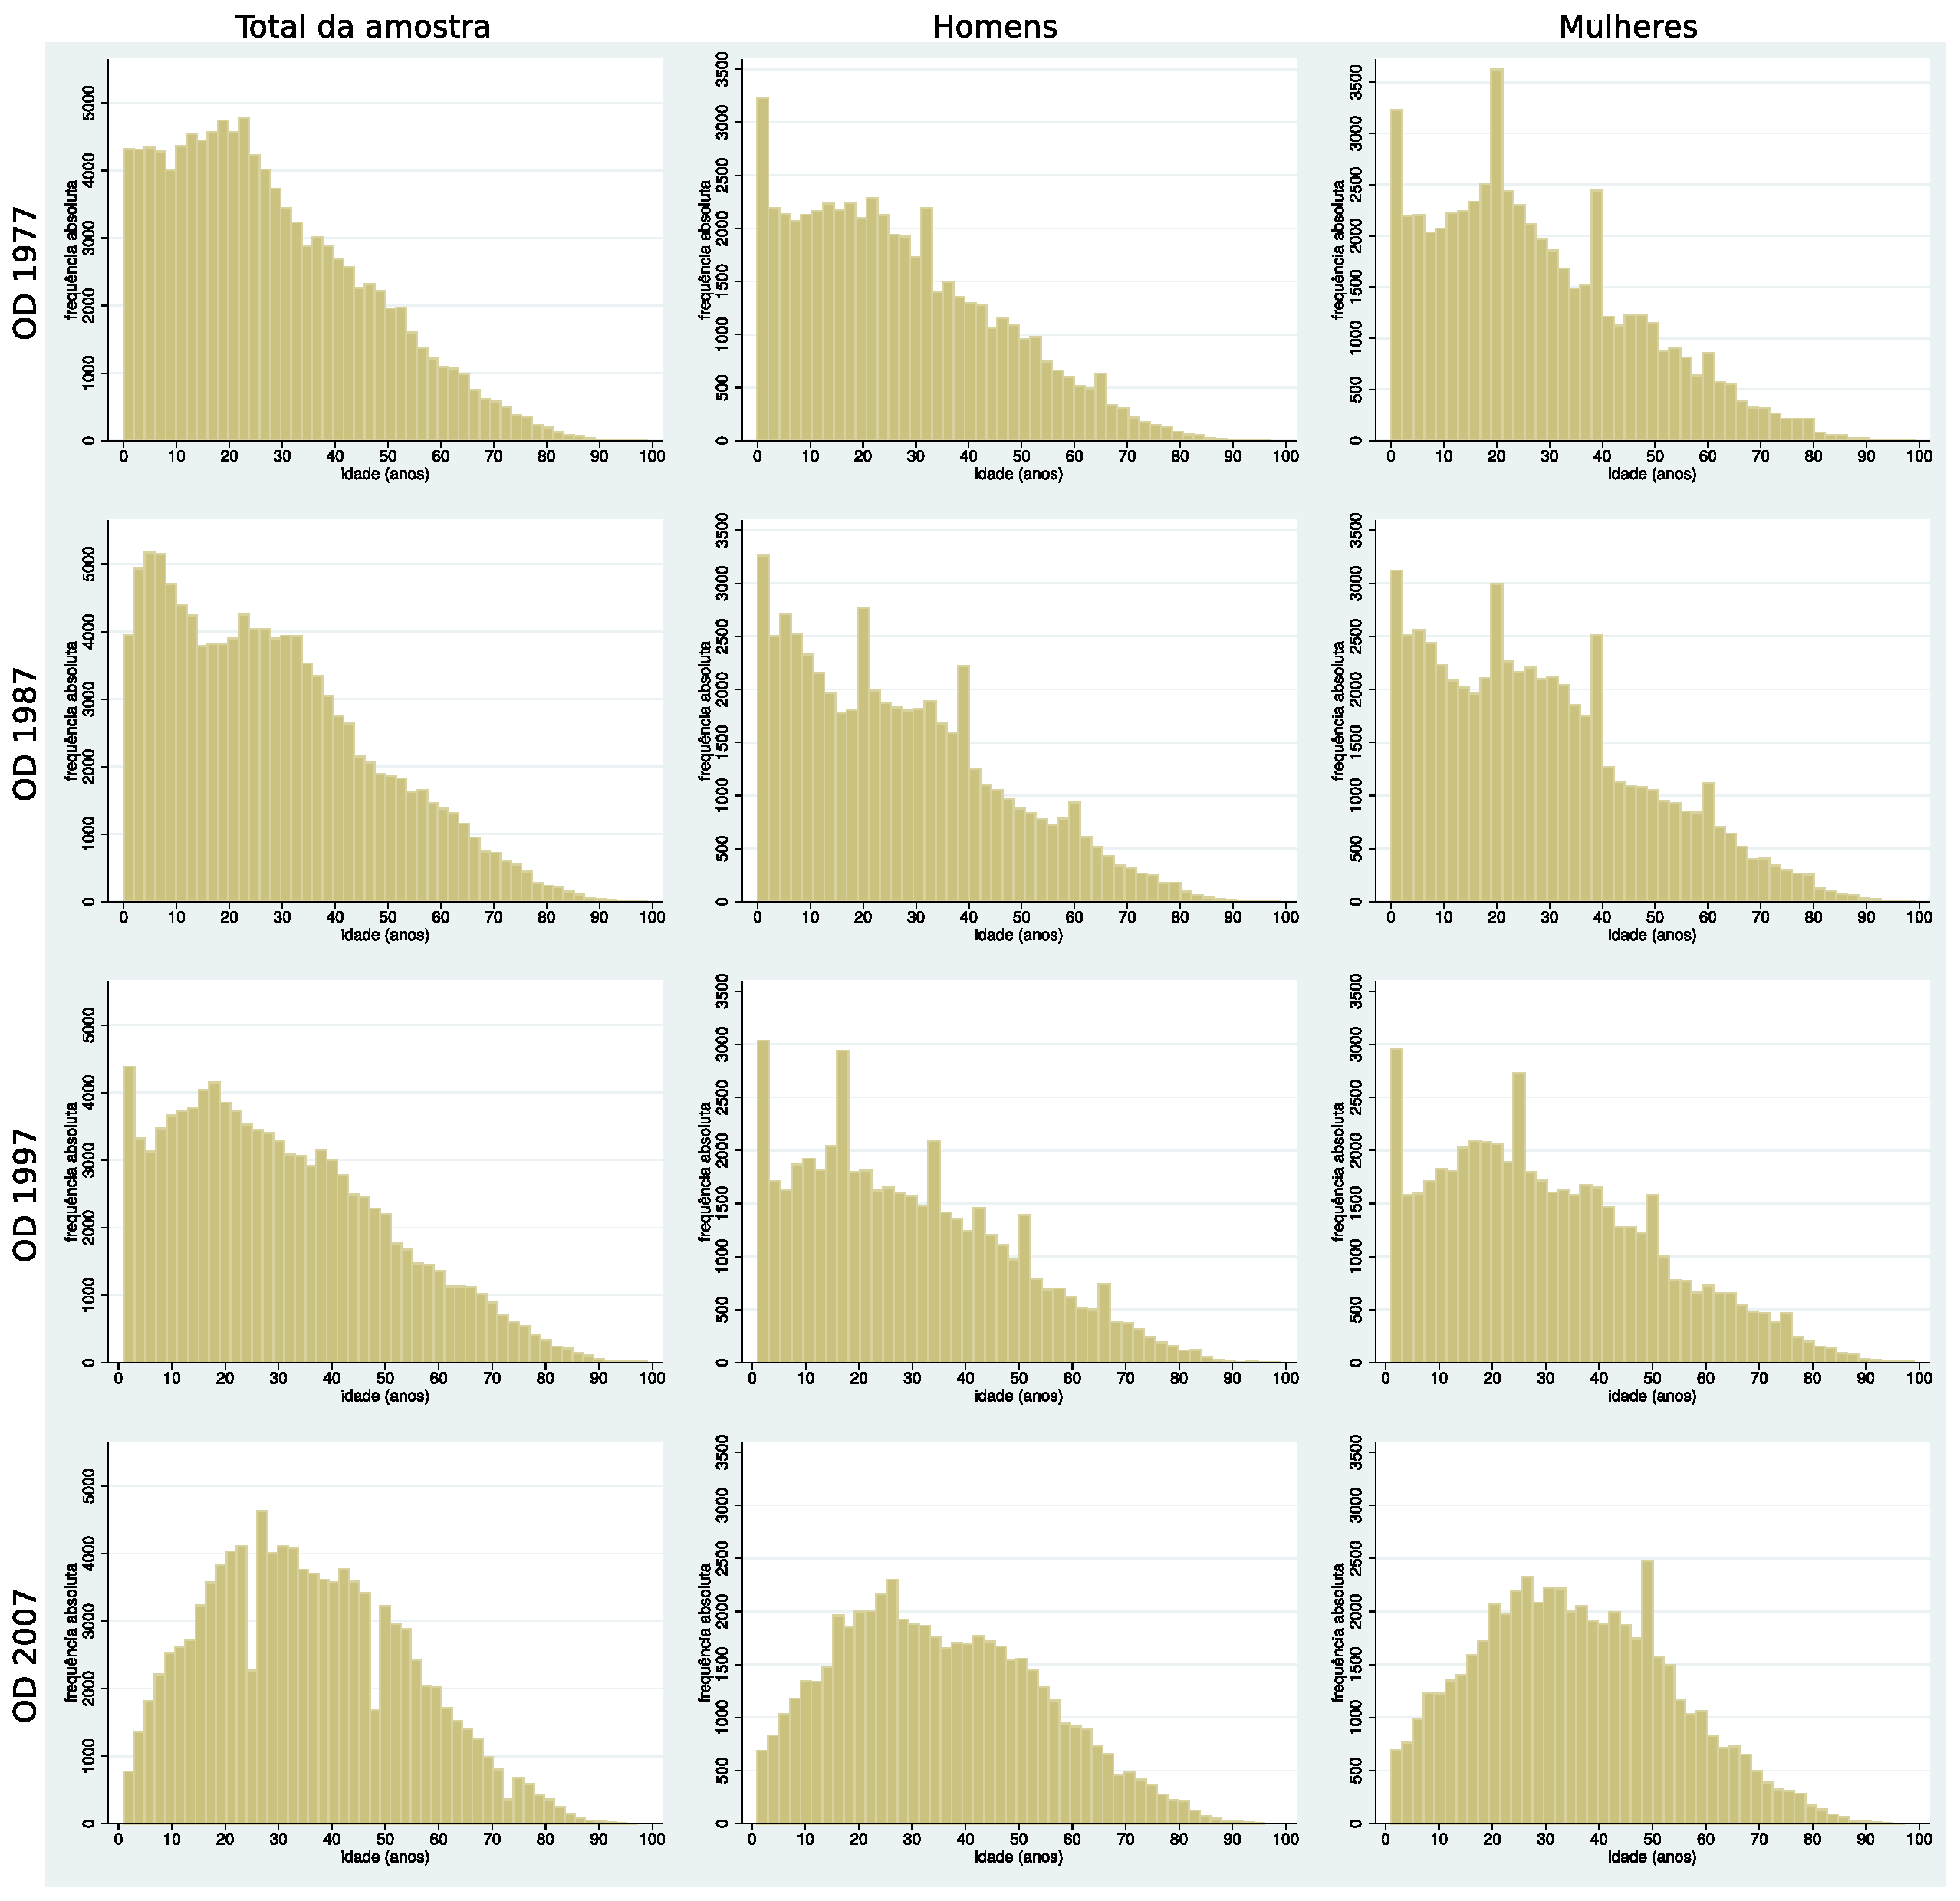
\includegraphics[width=1\textwidth]{./imagens/idade2.eps}%
    \end{center}%
    \fonte{Compilação própria}
\end{grafico}%

\clearpage
No Gráfico \ref{graf:distr-sit-fam} nota-se que para as mulheres houve uma mudança ao longo dessas três décadas. Em 1977, era mais frequente elas ocuparem a posição de filhas (41,81\%), em seguida de cônjuges (36,27\%). A posição de ``pessoa responsável'' pela família é a quarta categoria mais frequente (6,32\%), de seis. Tal distribuição permanace semelhante em 1987. Em 1997, no entanto, a posição de ``pessoa responsável'' pela família (11,13\%) já quase se equipara à posição de ``outro parente/agregado(a)'' (11,27\%). Em 2007, já é quase um quarto das mulheres entrevistadas que são responsáveis por suas famílias (24,21\%), representando aumento de quase 4 vezes em relação aos perecentuais de 1977. O percentual de mulheres cônjuges/companheiras pouco se altera ao longo do tempo, permanecendo na faixa dos 35\%. Há diminuição da posição de empregado(a) doméstico(a) para ambos sexos, mas a queda é mais acentuada para mulheres (da ordem de 8 vezes entre 1977 e 2007) do que para homens (queda em 2007 para cerca da metade do valor de 1977). Existe, também, queda da frequência daqueles que declaram-se na posição de filho(a) ou enteado(a) tanto para homens como para mulheres - em ordem de grandeza próxima: cerca de 8\% para mulheres e 10\% para homens. Isso pode ser reflexo da diminuição das taxas de fecundidade
\footnote{Por ``taxa de fecundidade total'' entende-se o número médio de filhos que teria uma mulher de uma coorte hipotética (15 e 49 anos de idade) ao final de seu período reprodutivo. Fonte: IBGE. Disponível em: \url{http://www.ibge.gov.br/home/estatistica/populacao/condicaodevida/indicadoresminimos/conceitos.shtm\#tf}} da população (ver Tabela \ref{tab:taxa-fecund}). Entre os homens percebe-se que houve crescimento entre aqueles com posição de ``pessoas responsável'' de cerca de 8\%, e também dos que declaram-se cônjuge/companheiro (cerca de 20 vezes) - esta última constatação é coerente com o fato de mais mulheres serem a principal fonte de renda doméstica, ou seja, a ``pessoa responsável'' da família.

\begin{table}[htb]
    \IBGEtab{%\renewcommand{\arraystretch}{1.5}%%\ABNTEXfontereduzida%
	    \renewcommand{\arraystretch}{1.5}
        \caption{Evolução das taxas de fecundidade no Brasil, de 1970 a 2010}
		\label{tab:taxa-fecund}
    }{%
	    \begin{tabular}{P{5.00cm} P{1.50cm} P{1.50cm} P{1.50cm} P{1.50cm} P{1.50cm}}
            \toprule
	           \headerTabCenterCell{Ano} &
   	           \headerTabCenterCell{1970} &
   	           \headerTabCenterCell{1980} &
   	           \headerTabCenterCell{1991} &
   	           \headerTabCenterCell{2000} &
   	           \headerTabCenterCell{2010} \\
		    \midrule \midrule
				Taxa de fecundidade (Brasil)&
				5,8&
				4,4&
				2,7&
				2,4&
		        1,9\\
			\midrule
				Taxa de fecundidade (Sudeste)&
				4,6&
				3,2&
				2,4&
				2,1&
		        1,7\\
			\midrule
				Taxa de fecundidade (São Paulo)&
				3,94&
				3,24&
				2,28&
				2,05&
		        1,67\\
			\bottomrule	
		\end{tabular}
    }{%
		\fonte{Compilação a partir de dados dos censos do IBGE disponíveis em \url{http://seculoxx.ibge.gov.br/populacionais-sociais-politicas-e-culturais/busca-por-palavra-chave/populacao/810-fecundidade} Acesso em 17 de novembro de 2014}
		\nota{Ao analisar as taxas de fecundidades para as Grandes Regiões, nota-se que o Sudeste tem os menores percentuais de mulheres que tiveram filhos em todos os subgrupos etários.}
		}
\end{table}

É possível que essa transformação dos papeis sociais desempenhados por homens e mulheres dentro do núcleo familiar ao longo das últimas décadas altere de maneira significativa os padrões de mobilidade de ambos grupos.

\clearpage

\begin{grafico}[htb]%
    \caption{\label{graf:distr-sit-fam}Distribuição da situação familiar de respondentes das Pesquisas OD 1977, 1987, 1997 e 2007, por sexo}%
    \begin{center}%
        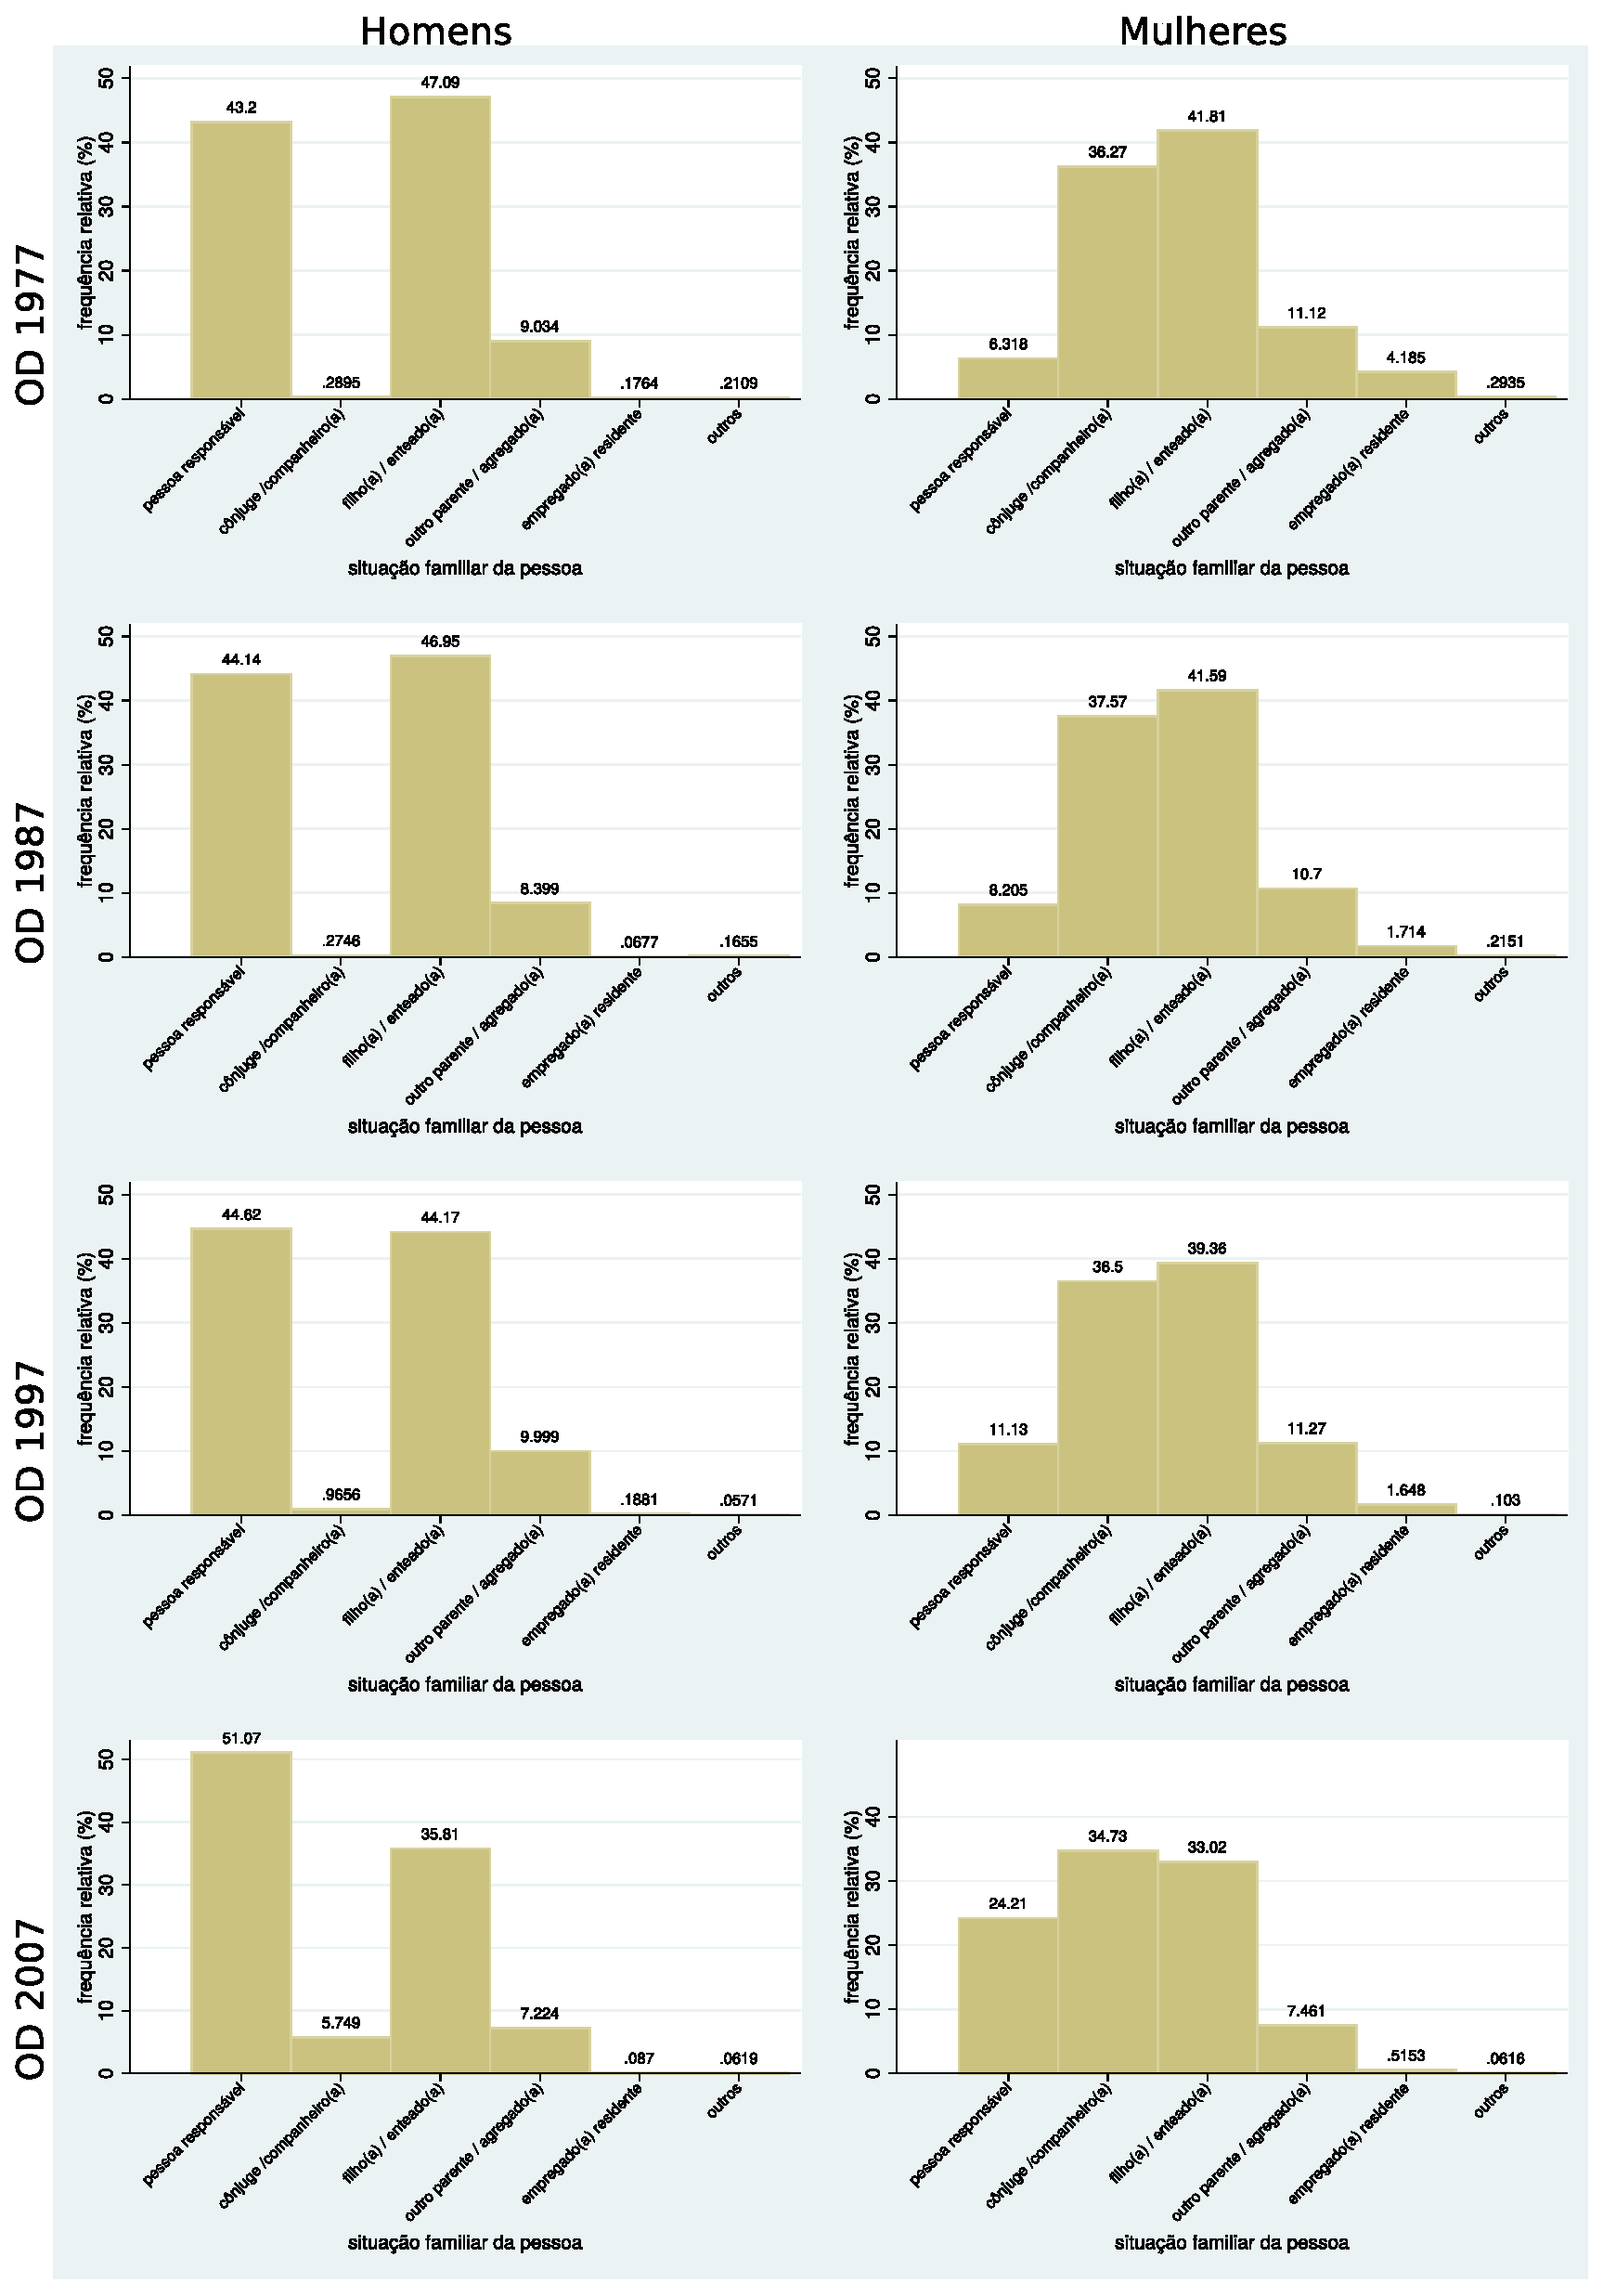
\includegraphics[width=1\textwidth]{./imagens/sitfam2.eps}%
    \end{center}%
    \fonte{Compilação própria}
\end{grafico}%

\clearpage

No Gráfico \ref{graf:distr-grau-instr} nota-se que em 1977 tanto homens como mulheres dispunham de pouco tempo de escolaridade - cerca de três quartos da população ou era analfabeta ou possuía no máximo o fundamental incompleto. Nessa época, nos três níveis de instrução superiores a esse os homens tinham índices maiores que as mulheres. O grau de instrução da população vai aumentando e em 1987, o grau de escolarização feminino é levemente superior ao masculino nas categorias ``fundamental completo / médio incompleto'' e ``médio completo / superior incompleto''. Na categoria ``superior completo'' o grau de instrução masculino é um pouco superior, situação que se inverte em 2007. Neste último ano de análise, as mulheres apresentam maiores percentuais nos dois níveis de maior grau de instrução e os homens, nos dois níveis de menor grau de instrução. Mesmo assim, as marcas para ambos são bastante semelhantes e indicam esforços de políticas públicas no sentido de universalizar os Ensinos Fundamental e Médio no Brasil \ref{tab:grau-instr-ef-em}.

\begin{table}[htb]
    \IBGEtab{%\renewcommand{\arraystretch}{1.5}%%\ABNTEXfontereduzida%
	    \renewcommand{\arraystretch}{1.5}
        \caption{Crescimento de matrículas no Ensino Fundamental e Ensino Médio, no Brasil, entre 1975 e 2005}
		\label{tab:grau-instr-ef-em}
    }{%
	    \begin{tabular}{P{2.00cm} P{4.00cm} P{4.00cm}}
            \toprule
	           \headerTabCenterCell{Ano} &
   	           \headerTabCenterCell{Matrículas no Ensino Fundamental} &
   	           \headerTabCenterCell{Matrículas no Ensino Médio}\\
		    \midrule \midrule
				1975&
		    	100*&
				100*\\
			\midrule
				1980&
				115,6&
		        113,1\\
			\midrule
				1990&
				141,0**&
		        180,8\\
			\midrule
				1996&
				169,5&
		        296,4\\
			\midrule
				2000&
				182,7&
		        423,2\\
			\midrule
				2005&
				171,5&
		        466,5\\
			\bottomrule	
		\end{tabular}
    }{%
		\fonte{Adaptado de \citeauthoronline{OLIVEIRA2007} (\citeyear{OLIVEIRA2007})}
		\nota{* Tomou-se por referência o ano de 1975 (1975=100). 
		** O valor refere-se ao ano de 1989.}
	}
\end{table}

O grau de instrução ter se elevado entre 1977 e 2007 influencia não apenas a empregabilidade e, eventualmente as viagens motivo trabalho. O principal impacto esperado desse fenômeno dá-se nas viagens motivo escola - realizadas por um contingente de pessoas cada vez maior, mais diverso e contendo mais faixas etárias.

\begin{grafico}[htb]%
    \caption{\label{graf:distr-grau-instr} Distribuição do grau de instrução de respondentes das Pesquisas OD 1977, 1987, 1997 e 2007, por sexo}%
    \begin{center}%
        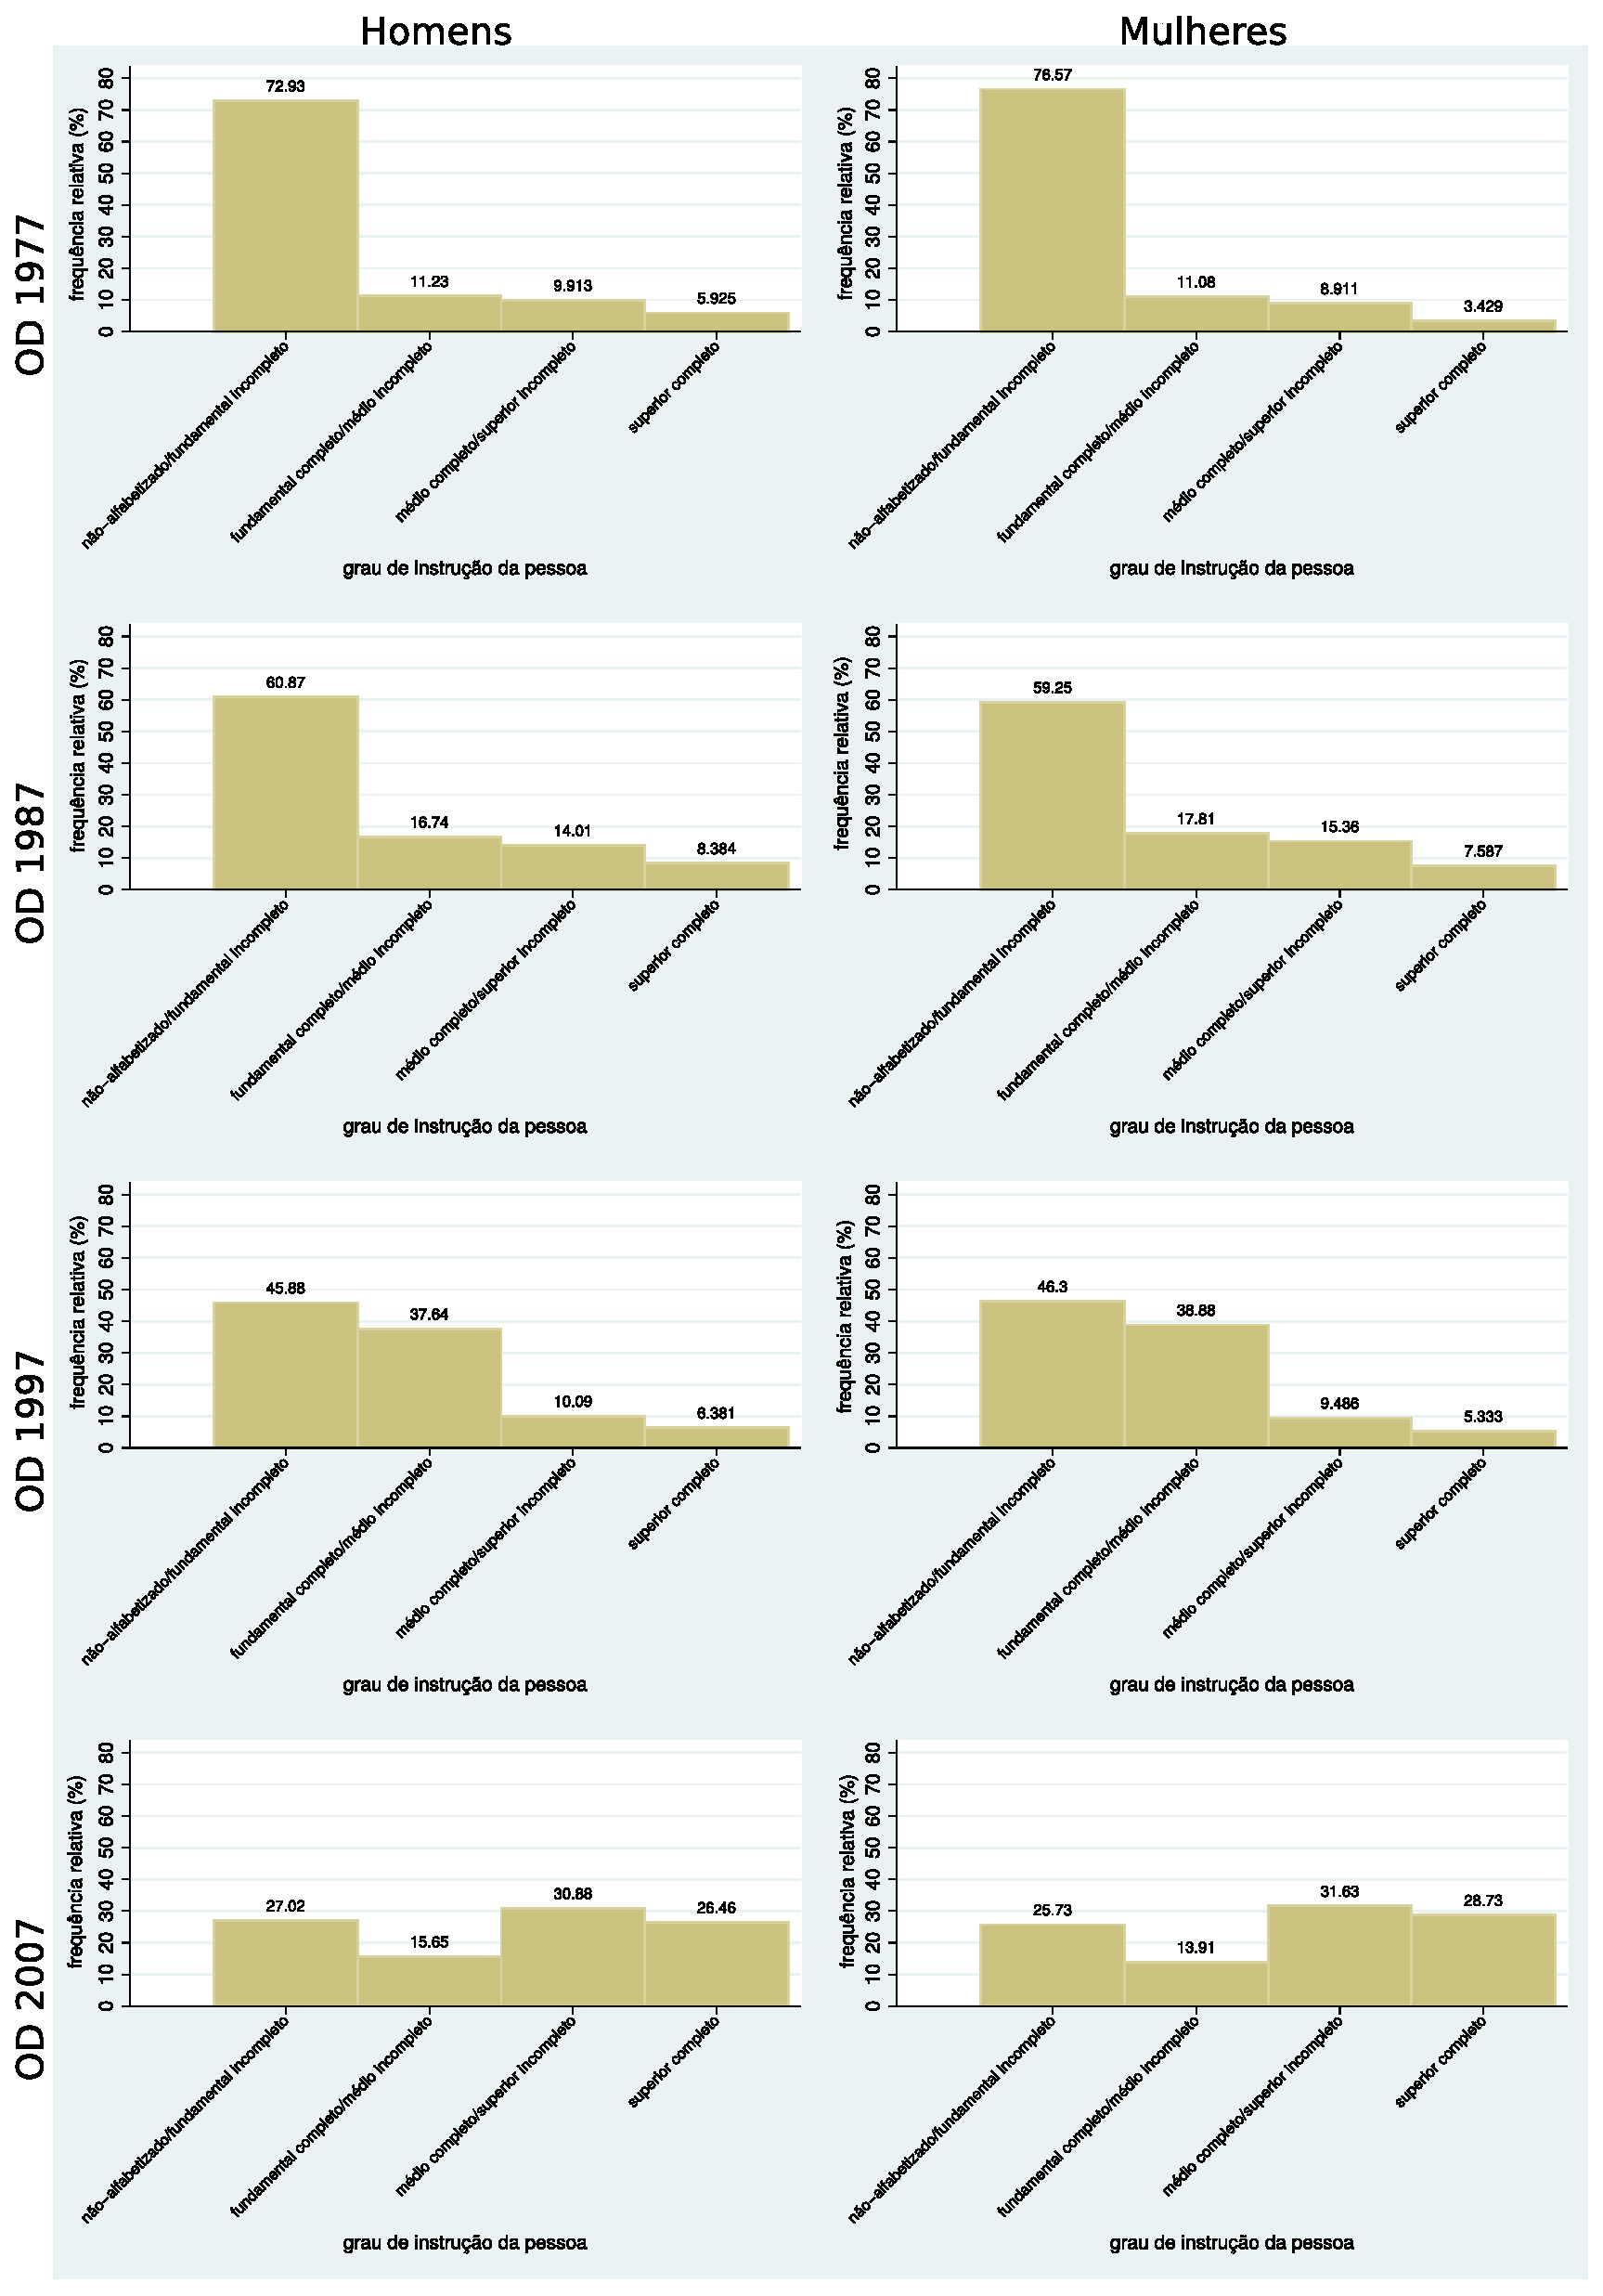
\includegraphics[width=1\textwidth]{./imagens/grauinstr2.eps}%
    \end{center}%
    \fonte{Compilação própria}
\end{grafico}%

\clearpage
Para atribuição da renda foram feitas regressões baseadas nos bens de consumo levantados.
Em 1977, foi adotado o critério \hl{XXX} e a equação \eqref{eq:reg-renda-77} explicita como foi feita a atribuição da renda.
Em 1987, foi adotado o critério ABA/ABIMEPE e a equação \eqref{eq:reg-renda-87} explicita como foi feita a atribuição da renda. 
Em 1997, foi adotado o critério ABIMEPE e a equação \eqref{eq:reg-renda-97} explicita como foi feita a atribuição da renda.
Em 2007, foi adotado o critério ABEP e a equação \eqref{eq:reg-renda-07} explicita como foi feita a atribuição da renda.

\hl{explicar como foi feito o cálculo da renda atribuída, para cada OD}

\hl{explicar como foram trazidos os valores para o valor presente (outubro de 2007)}

\begin{equation}\label{eq:reg-renda-1997}
RFM = e^{~5,672~+~0,03259*PONT}
\end{equation}

\begin{equation}\label{eq:reg-renda-2007}
RFM = e^{~5,864~+~0,084*PONT}
\end{equation}

\hl{fazer essas transformações no banco e rodar análises f(rend\_ind) e f(renda\_fam)}

\clearpage
Este grupo de análises que se segue busca compreender como essa amostra se comporta em termo de viagens realizadas, em cada ano e diferencialmente entre os anos, olhando para tanto variáveis como duração das viagens e número de viagens realizadas.

%Dentro deste segundo grupo de análises foi de interese buscar verificiar se a variável explicativa sexo era relevante para explicar tanto a duração como o número de viagens. Para tanto foram feitas regressões lineares simples e seus resultados são apresentados na Seção \ref{sec:analises-preliminares}. Também há interesse em verificar se existe alguma diferença estatisticamente significativa nos padrões de deslocamento entre os sexos, para cada \emph{cross-section}. Isso foi feito feito tomando como hipótese nula que as médias de ambos sexos eram iguais, para as variáveis dependentes analisadas. Essa hipótese foi testada e os resultados também são apresentados na Seção \ref{sec:analises-preliminares}.

O Gráfico \ref{graf:distr-dur-viag} foi construído considerando-se apenas as vigens cuja duração fosse igual ou superior a 5 minutos. Em todos anos, para homens e para mulheres, percebem-se alguns picos que ocorrem nos valores múltiplos de cinco minutos. Isso porque a duração expressa trata-se da duração de viagem percebida e declarada pelo(a) respondente. Em 1977, a duração das viagens mais curtas (como 5 e 30 minutos) era menos frequente entre as mulheres (13\% e 14\%, respectivamente) do que entre os homenso (26\% e 15\%). No mesmo ano, as viagens mais longas eram mais frequentes entre as mulheres (5\% para 60 minutos e 2\% para 90 minutos) do que entre os homens (6,5\% para 60 minutos e 3\% para 90 minutos). De 1987 as viagens de 5 minutos passam a ser mais frequentes entre mulheres (32\%) do que entre homens (26,5\%). Essa sitação se inverte em 1997 e retorna em 2007.
Em todas anos as viagens mais longas (de 60 e 90 minutos) São mais frequentes entre os homens do que entre as mulheres.
Na Tabela \ref{tab:dur-med-viag} são apresentadas as durações médias de viagens para homens e mulheres. As médias de homens são superiores às das mulheres, ao nível de significância estatística de 5\%. É possível perceber que a duração média de viagem para ambos vem crescendo e a diferença entre esses grupos vem diminuindo.

\hl{verificar se é preiso apresentar os resultados de teste F e teste t p/ comparação de médias OU ANOVA com prévia averiguaçaõ de matrizes de covariância + teste Levene + teste normalidade (não vai passar...)}

\begin{table}[htb]
    \IBGEtab{%\renewcommand{\arraystretch}{1.5}%%\ABNTEXfontereduzida%
	    \renewcommand{\arraystretch}{1.5}
        \caption{Duração média de viagem, por sexo, por ano}
		\label{tab:dur-med-viag}
    }{%
	    \begin{tabular}{P{1.50cm} P{2.00cm} P{2.00cm} P{3.00cm} P{3.00cm} P{3.00cm}}
            \toprule
	           \headerCenterCell{Ano} &
   	           \headerCenterCell{Duração Média de Viagem para Mulheres (min)} &
   	           \headerCenterCell{Duração Média de Viagem para Homens (min)} &
   	           \headerCenterCell{Desvio Padrão da Duração Média de Viagem para Mulheres}&   	           
   	           \headerCenterCell{Desvio Padrão da Duração Média de Viagem para Homens} &   	           
   	           \headerCenterCell{Diferença entre as durações médias (Dur\_mulher - Dur\_homem)}\\
		    \midrule \midrule
				1977&
		    	29,23&
		    	33,27&
		    	28,52&
		    	31,69&
				-4,04\\
			\midrule
				1987&
				30,27&
				35,82&
				29,29&
				33,11&
		        -5,55\\
			\midrule
				1997&
				32,09&
				35,61&
				30,83&
				33,90&
		        -3,52\\
			\midrule
				2007&
				35,35&
				37,39&
				32,76&
				33,87&
		        -2,04\\
			\bottomrule	
		\end{tabular}
    }{%
		\fonte{Elaboração própria}
	}
\end{table}

Ao fazer a regressão linear da variável duração (valores superiores a 5 minutos) unicamente em função da variável explicativo sexo, para todos anos os p-valores foram inferiores a 0,05, o que mostra indícios de que a variável sexo é umas das variáveis de análise para explicar o tempo dispendido nos deslocamentos.

\begin{grafico}[htb]%
    \caption{\label{graf:distr-dur-viag}Distribuição da duração de viagens de respondentes das Pesquisas OD 1977, 1987, 1997 e 2007, por sexo}%
    \begin{center}%
        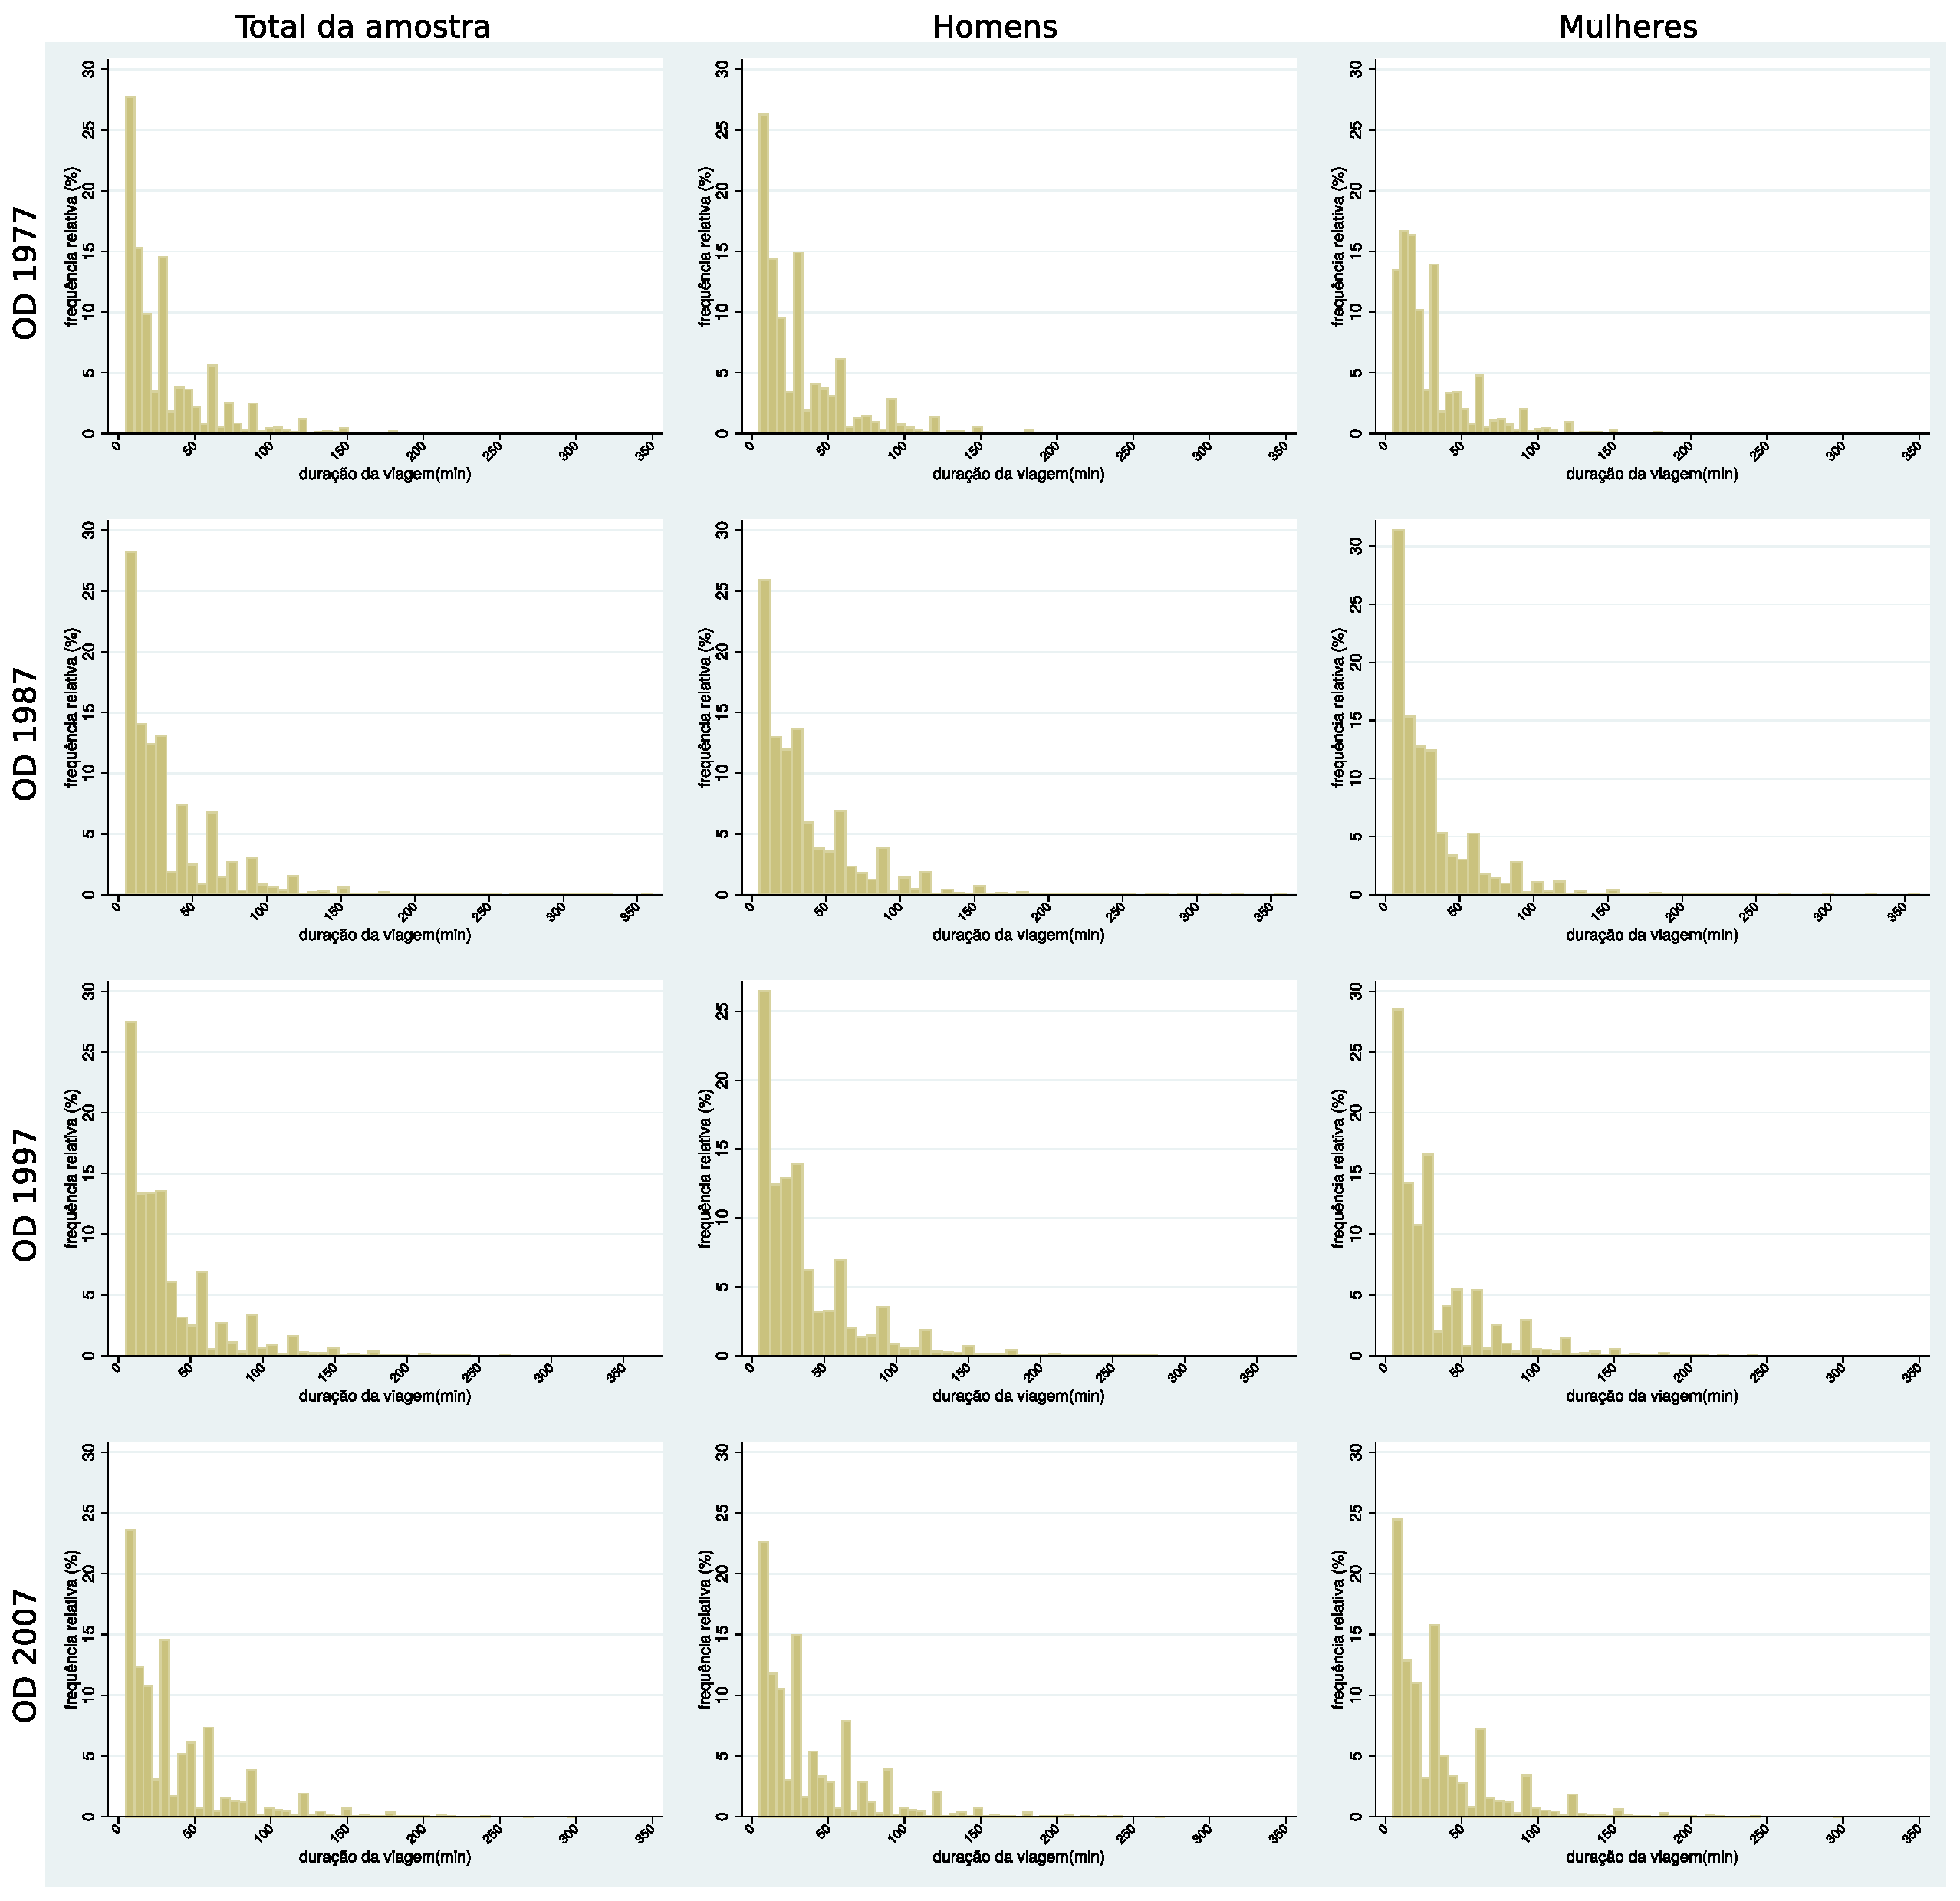
\includegraphics[width=1.1\textwidth]{./imagens/duradeviagens2.eps}%
    \end{center}%
    \fonte{Compilação própria}
\end{grafico}%

\clearpage
Analisando a dsitribuição do número de viagens por pessoa, conforme já era de se esperar, para quem faz viagem (número de viagem é não nulo) existe a predominância do valor 2, o que indica que é caracaterístico de pessoas que trabalham ou que estudam, pois saem da sua residência com esse propósito (que ocupa a maior parte do seu dia) e depois retornam à residência apśoa atividade. O que vale analisar no Gráfico \ref{graf:distr-num-viag} é a relação entre as viagens nulas (não sai de casa) e as viagens de idae volta (valores iguais a 2). Para homens, o número de viagens nulo é menos frequente que o número de viagens de valor 2 para todos anos de análise. Já para as mulheres, em 1977 as viagens nulas eram a maioria, indicando certa fixitude delas. Essa porcentagem vai diminuido e a porcentagem no número de viagens igual a 2 vai crescendo, ficam próximas em 1997 e, em 2007, inverte-se a situação observada em 1977. Coincidentemente com a conquista de maior participação no mercado de trabalho, essa alteração pode ser indícios de que as mulheres ganharam mobilidade, restringindo-se menos ao espaço doméstico.

Na Tabela \ref{tab:num-med-viag} são apresentados os números médios de viagens para homens e mulheres. As médias de homens são superiores às das mulheres, ao nível de significância estatística de 5\%. O número médio de viagens para os homens caiu entre 1977 e 1997, voltando a subir em 2007. \hl{pq??} O número médio de viagens para as mulheres aumntou desde 1977 até 2007. Apesar dessa mudança de tendência no padrão masculino, a diferença entre os gêneros só tem diminuido.

Ao fazer a regressão linear da variável total de viagens da pessoa (para o primeiro registro da pessoa) unicamente em função da variável explicativo sexo, para todos anos os p-valores foram inferiores a 0,05, o que mostra indícios de que a variável sexo é umas das variáveis de análise para explicar a quantidade de viagens feitas pelo indivíduo.

%\hl{verificar se é preciso apresentar os resultados de teste F e teste t p/ comparação de médias OU ANOVA com prévia averiguaçaõ de matrizes de covariância + teste Levene + teste normalidade (não vai passar...)}

\begin{table}[htb]
    \IBGEtab{%\renewcommand{\arraystretch}{1.5}%%\ABNTEXfontereduzida%
	    \renewcommand{\arraystretch}{1.5}
        \caption{Número médio de viagens, por sexo, por ano}
		\label{tab:num-med-viag}
    }{%
	    \begin{tabular}{P{1.00cm} P{2.00cm} P{2.00cm} P{3.00cm} P{3.00cm} P{3.50cm}}
            \toprule
	           \headerCenterCell{Ano} &
   	           \headerCenterCell{Número Médio de Viagem para Mulheres (min)} &
   	           \headerCenterCell{Número Médio de Viagem para Homens (min)} &
   	           \headerCenterCell{Desvio Padrão da Número Médio de Viagem para Mulheres} &   	           
   	           \headerCenterCell{Desvio Padrão do Número Médio de Viagem para Homens} &   	           
   	           \headerCenterCell{Diferença entre os números médios de viagens (Nº\_viag\_mulher - Nº\_viag\_homem)}\\
		    \midrule \midrule
				1977&
		    	1,40&
		    	2,09&
		    	1,64&
		    	1,92&
				-0,69\\
			\midrule
				1987&
				1,42&
				1,89&
				1,59&
				1,61&
		        -0,47\\
			\midrule
				1997&
				1,53&
				1,79&
				1,63&
				1,60&
		        -0,26\\
			\midrule
				2007&
				1,75&
				1,98&
				1,64&
				1,58&
		        -0,23\\
			\bottomrule	
		\end{tabular}
    }{%
		\fonte{Elaboração própria}
	}
\end{table}


\begin{grafico}[htb]%
    \caption{\label{graf:distr-num-viag}Distribuição do número de viagens por respondente das Pesquisas OD 1977, 1987, 1997 e 2007, por sexo}%
    \begin{center}%
        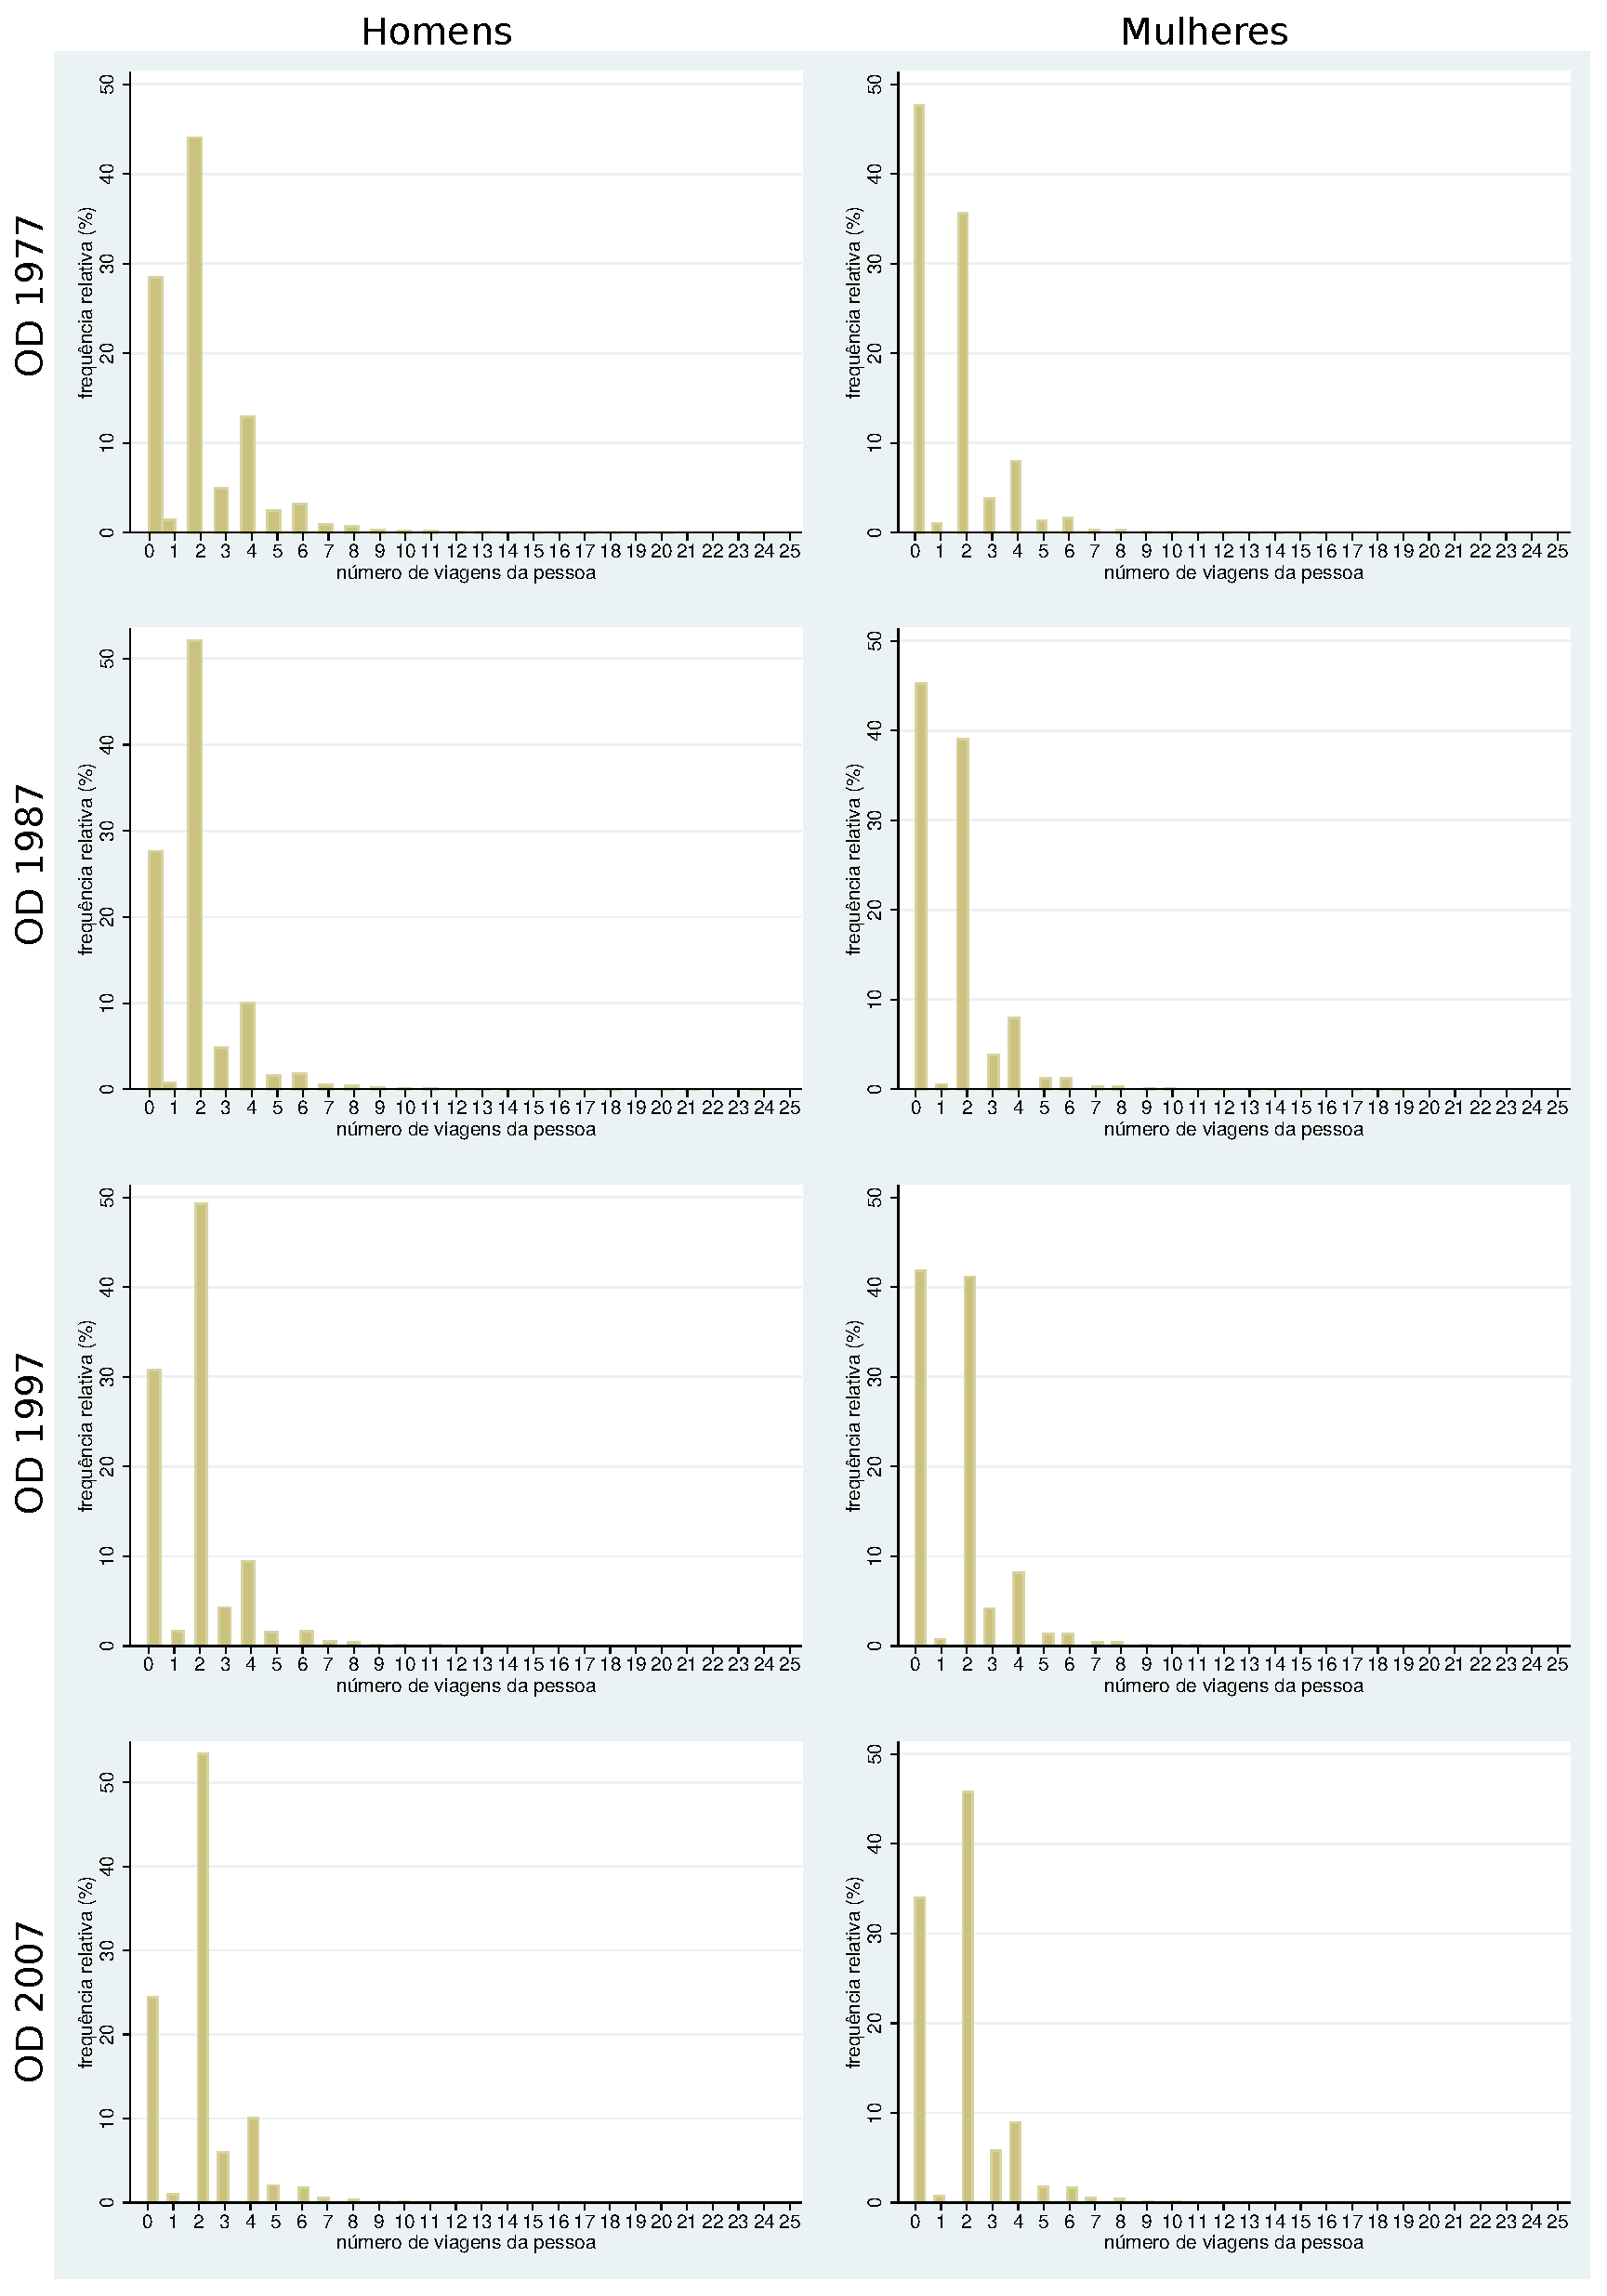
\includegraphics[width=1\textwidth]{./imagens/qtdeviagens2.eps}%
    \end{center}%
    \fonte{Compilação própria}
\end{grafico}%

